\documentclass{beamer}

\usetheme[progressbar=head, block=fill]{metropolis}
\usepackage[utf8]{inputenc}
\usepackage[makeroom]{cancel}
\usepackage{amsmath}

\usepackage{svg}

\usepackage{amsmath}
\usepackage{amsfonts}
\usepackage{mathtools}

\usepackage{siunitx} 

\usepackage{color}
\usepackage{manfnt}
\usepackage{graphicx}
\usepackage[dvipsnames]{xcolor}
\definecolor{dgreen}{rgb}{0,0.6,0}
\usepackage{amssymb}
\usepackage{pifont}
\usepackage{mathtools}
\usepackage{multimedia}
\usepackage{media9}
\usepackage{centernot}
\usepackage{amsthm}

% listening
\definecolor{bluekeywords}{rgb}{0.13,0.13,1}
\definecolor{greencomments}{rgb}{0,0.5,0}
\definecolor{redstrings}{rgb}{0.9,0,0}
\usepackage{listings}
\lstset{language=C,
  showspaces=false,
  showtabs=false,
  breaklines=true,
  showstringspaces=false,
  breakatwhitespace=true,
  escapeinside={(*@}{@*)},
  commentstyle=\color{greencomments},
  keywordstyle=\color{bluekeywords},
  stringstyle=\color{redstrings},
  basicstyle=\fontsize{9}{11}\ttfamily,
  keywords=[2]{int32},
  keywordstyle=[2]{\color{bluekeywords}},
  keywords=[3]{uint8},
  keywordstyle=[3]{\color{bluekeywords}},
  keywords=[4]{uint16},
  keywordstyle=[4]{\color{bluekeywords}},
  keywords=[5]{uint32},
  keywordstyle=[5]{\color{bluekeywords}}
}

\graphicspath{ {figures/} }

\renewcommand{\vec}[1]{\boldsymbol{#1}}
\newcommand{\matr}[1]{\mathbf{#1}}
\newcommand{\cmark}{\ding{51}}%
\newcommand{\xmark}{\ding{55}}%

\newcommand{\unitvec}[1]{\hat{\boldsymbol{#1}}}
\newcommand{\transpose}{^{\mathrm{T}}}

\date{xx/09/2017}

\title[]{xxxxx}
\subtitle{Corso di LM in Ingegneria Robotica ed Automazione \\
  Sistemi di Guida e Navigazione}
\author{Studenti:\hfill Supervisore:\\
Nicola Piga \hfill Prof. Lorenzo Pollini\\
Giulio Romualdi}
\institute[]{Università di Pisa}
\begin{document}
%\beamertemplatenavigationsymbolsempty

\begin{frame}
  \maketitle
\end{frame}

\section{Descrizione dei contenuti}
\begin{frame}{Contenuti}
  \begin{itemize}
  \item [-] Descrizione del funzionamento di base del sistema DecaWave EVB1000
  \item [-] Descrizione dell'implementazione originale del firmware
  \item [-] Descrizione della procedura originale di ranging tra le ancore 
  \item [-] Implementazione della nuova procedura di autoranging
  \item [-] Guida al codice sviluppato
  \item [-] Implementazione di un Viewer per la visualizzazione di posizione ed assetto del Tag
  \item [-] Esempi di postprocessing e visualizzazione dati con MATLAB
  \end{itemize}
\end{frame}

\section{Funzionamento di base del sistema DecaWave EVB1000}
\begin{frame}{Introduzione}
  Il sistema di tag ed ancore DecaWave EVB1000 consente di localizzare
  un agente attraverso ricetrasmettitori che implementano la tecnica di trasmissione
  \alert{UWB} (Ultra-wideband).\\
  Alla base del funzionamento del sistema vi è lo scambio di messaggi, tra tag e ancore,
  contententi principalmente informazioni di natura temporale. Tali informazioni consentono
  alle ancore di calcolare il tempo di volo tra esse e il tag e quindi, mediante opportuno
  algoritmo di trialaterazione, di calcolare la posizione del tag.
\end{frame}

\begin{frame}{Two-way Ranging}
  Lo scambio di messaggi avviene secondo il metodo detto \alert{Two-way Ranging}.\\
  Nel dettaglio vengono scambiati, tra tag e ciascuna ancora,
  un messaggio di Poll, uno di Risposta ed uno di Final.\\
  I messaggi di \alert{Poll} e \alert{Final} vengono inviati dal tag
  mentre ogni ancora invia il messaggio di \alert{Risposta}.
  \begin{center}
    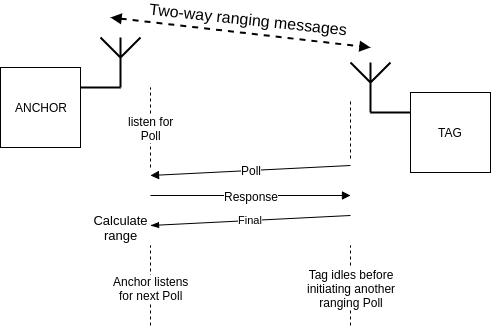
\includegraphics[height=10em]{ranging.png}
  \end{center}
\end{frame}

\begin{frame}{Struttura di un messaggio ed RMARKER}
  La struttura dei messaggi scambiati da tag e ancore è la seguente.
  \begin{center}
    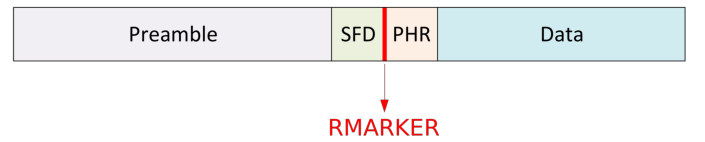
\includegraphics[width=\linewidth]{whole_msg_decawave}
  \end{center}
  Il campo \alert{Data} contiene i dati veri e propri scambiati tra i dispositivi.\\
  Durante la trasmissione di un messaggio l'inizio della parte PHR (PHY header)
  costituisce l'evento da utilizzare per il time-stamping come da standard
  IEEE 802.15.4 UWB PHY. Il tempo, espresso nell'orologio locale del dispositvo, di invio
  del primo simbolo del PHR sarà definito nel seguito \alert{RMARKER}.
\end{frame}

\begin{frame}{Two-way Ranging}
  \begin{columns}[T]
    \begin{column}{0.5\textwidth}
      il \alert{tag} salva RMARKER di
      \begin{itemize}
      \item[-] invio Poll ($Rm_{ps}$)
      \item[-] ricezione Risposta ($Rm_{rr}$)
      \item[-] invio Final ($Rm_{fs}$) (delayed transmission)
      \end{itemize}
    \end{column}
    \begin{column}{0.5\textwidth}
      l'\alert{ancora} salva RMARKER di
      \begin{itemize}
      \item[-] ricezione Poll ($Rm_{pr}$)
      \item[-] spedizione Risposta ($Rm_{rs}$)
      \item[-] ricezione Final ($Rm_{fr}$)
      \end{itemize}
    \end{column}
  \end{columns}
  \begin{center}
    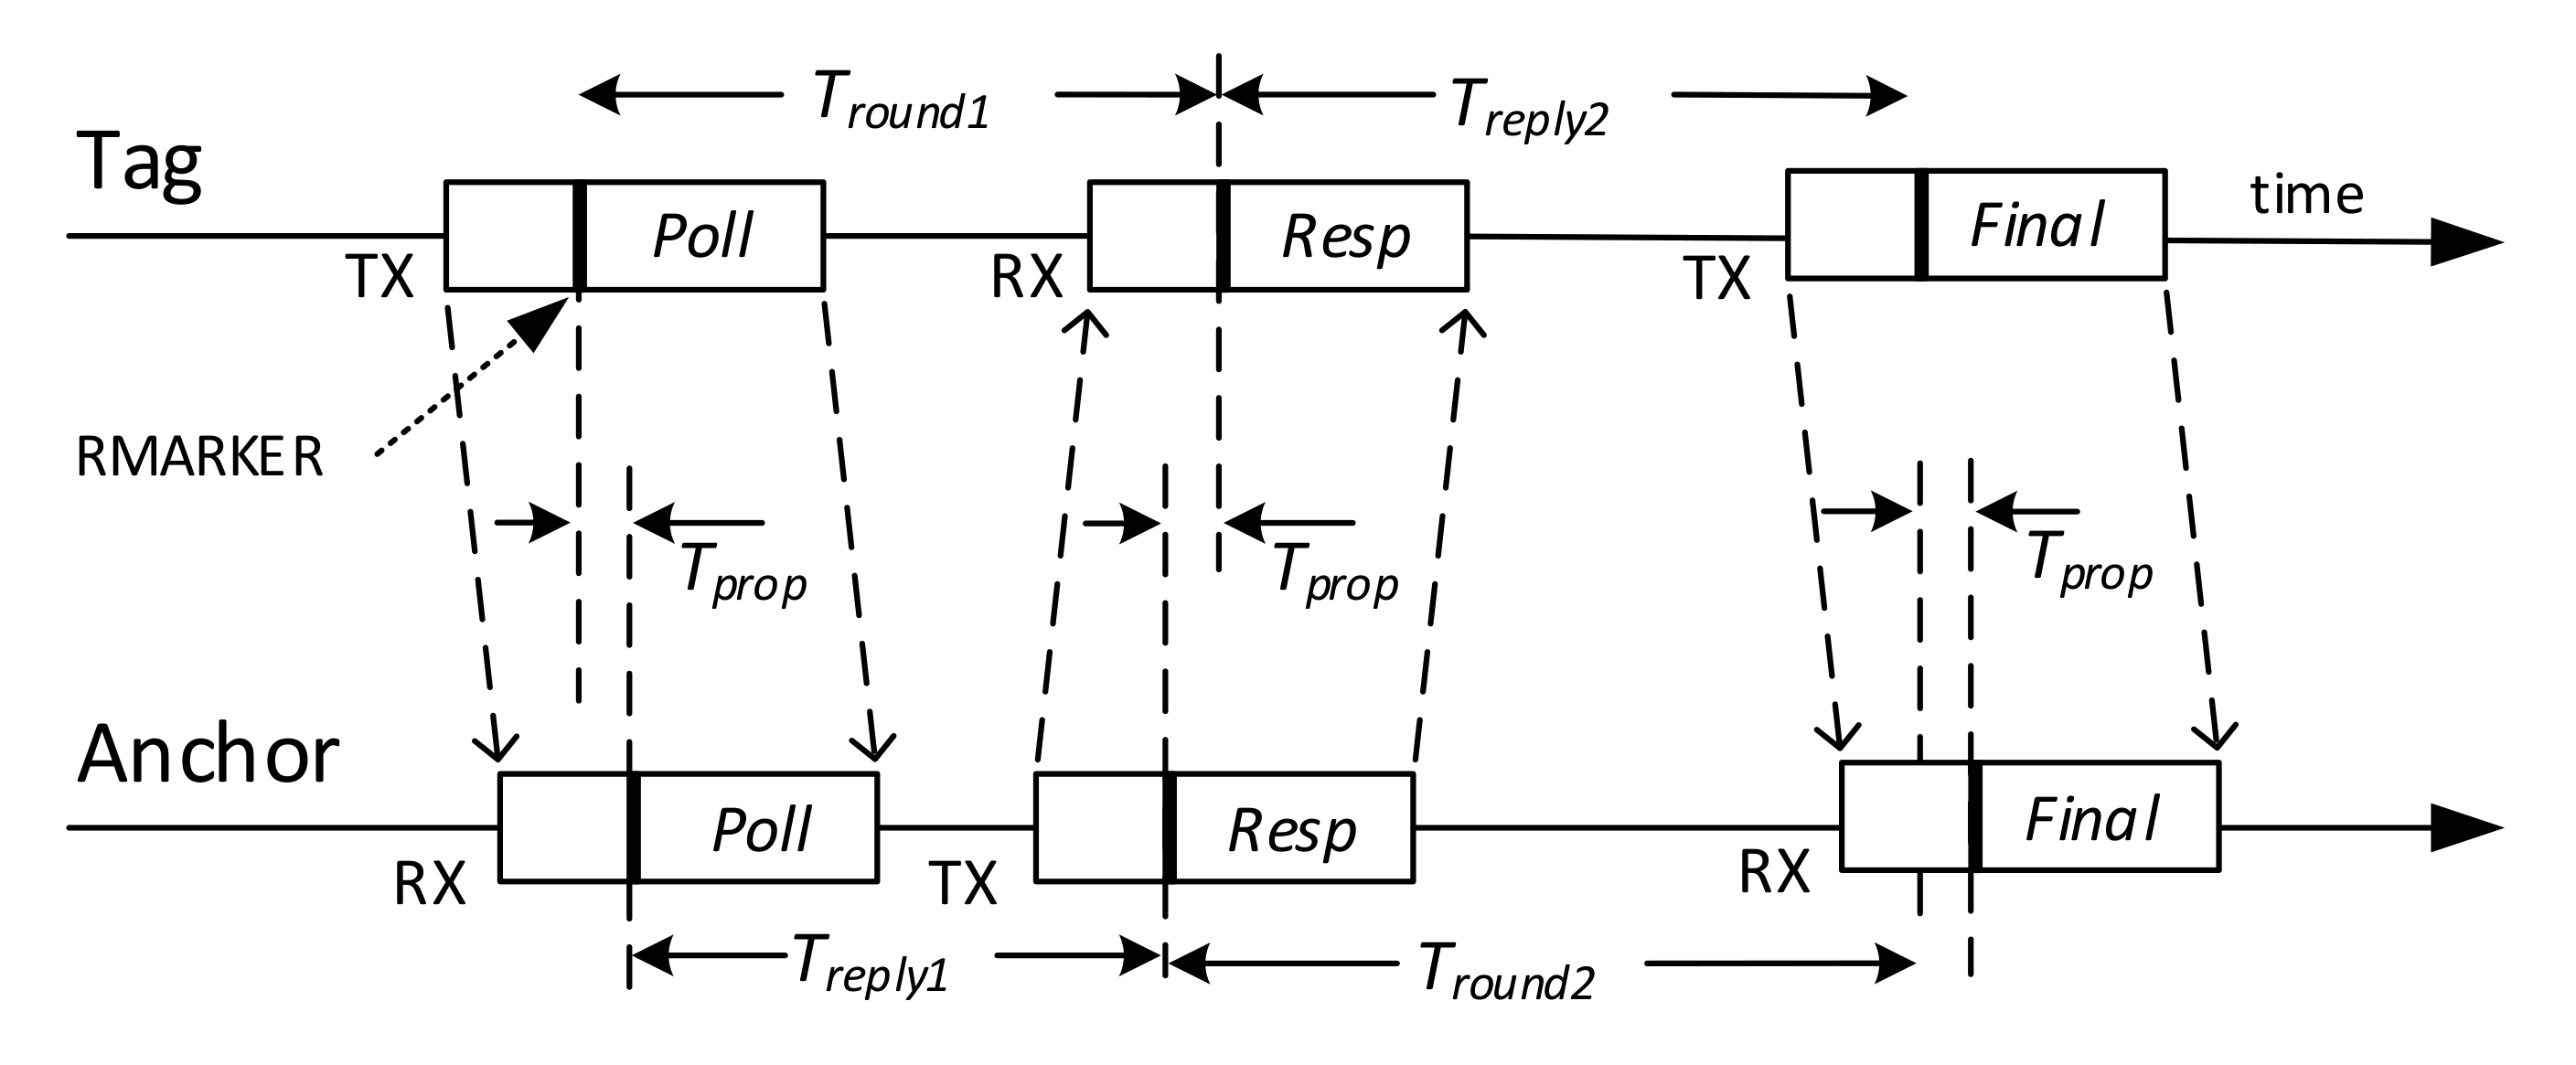
\includegraphics[scale = 0.7]{ranging_with_timings.png}
  \end{center}
  Il tag invia $Rm_{ps}$, $Rm_{rr}$ e $Rm_{fs}$ all'ancora nel Final.
\end{frame}

\begin{frame}{Calcolo del ToF}
  Le seguenti quantità sono \alert{calcolate} dall'\alert{ancora} utilizzando i dati raccolti e
  ricevuti dal tag durante un'istanza di ranging
  \[
  \begin{split}
    T_{round1} = Rm_{rr} - Rm_{ps} \quad \quad T_{round2} = Rm_{fs} - Rm_{rr}\\
    T_{reply1} = Rm_{rs} - Rm_{pr} \quad \quad T_{reply2} = Rm_{fr} - Rm_{rs}
  \end{split}
  \]

  Alla ricezione del Final l'ancora calcola il nuovo Tof ($T_{prop}$) che viene inviato al tag nella Risposta al Poll dell'istanza di ranging \alert{successiva}
  \[
  T_{prop} = \frac{T_{round1} T_{round2} - T_{reply1} T_{reply2}}{T_{round1} + T_{round2} + T_{reply1} + T_{reply2}}
  \]
\end{frame}

\begin{frame}[label={delayed_tx}]{Delayed transmission}
  \begin{alertblock}{Attenzione}
    La necessità di spedire nel messaggio di Final il tempo di spedizione del medesimo richiede
    l'utilizzo della funzione di \emph{delayed transmission} del DW1000.
  \end{alertblock}
  Il tempo di spedizione viene scelto a priori come
  \[
  Rm_{fs} = Rm_{ps} + T_{fd}
  \]
  dove $T_{fd}$ è maggiore del tempo impiegato da \alert{tutte le ancore} per rispondere al tag ed è indicato
  con Final Delay.
  La funzione di \emph{delayed transmission} garantisce che l'RMARKER di spedizione del Final coincida con
  $Rm_{fs}$.
\end{frame}

\begin{frame}{Superframe e frame}
  Durante la trasmissione dei dati i tag e le ancore osservano un protocollo di trasmissione
  \alert{a divisione di tempo} per evitare che un dispositivo possa interferire con la trasmissione
  di un altro.\\
  Nel dettaglio il tempo è diviso in una serie di \alert{superframe} a loro volta divisi in
  frame.\\
  Il firmware originale prevede 10 frame della durata di \SI{10}{\milli\second}, otto dei quali
  sono dedicati ad altrettante istanze di ranging, una per ciascun tag. I restanti due sono dedicati
  alla ``vecchia'' procedura di ranging tra le ancore. In totale ciascun superframe ha un durata di \SI{100}{\milli\second}.\\
  La configurazione del firmware originale prevede fino a $8$ tag e $3$/$4$ ancore.
\end{frame}

\begin{frame}{Esempio di temporizzazione}
  Un esempio di temporizzazione è mostrato di seguito.
  \centering
  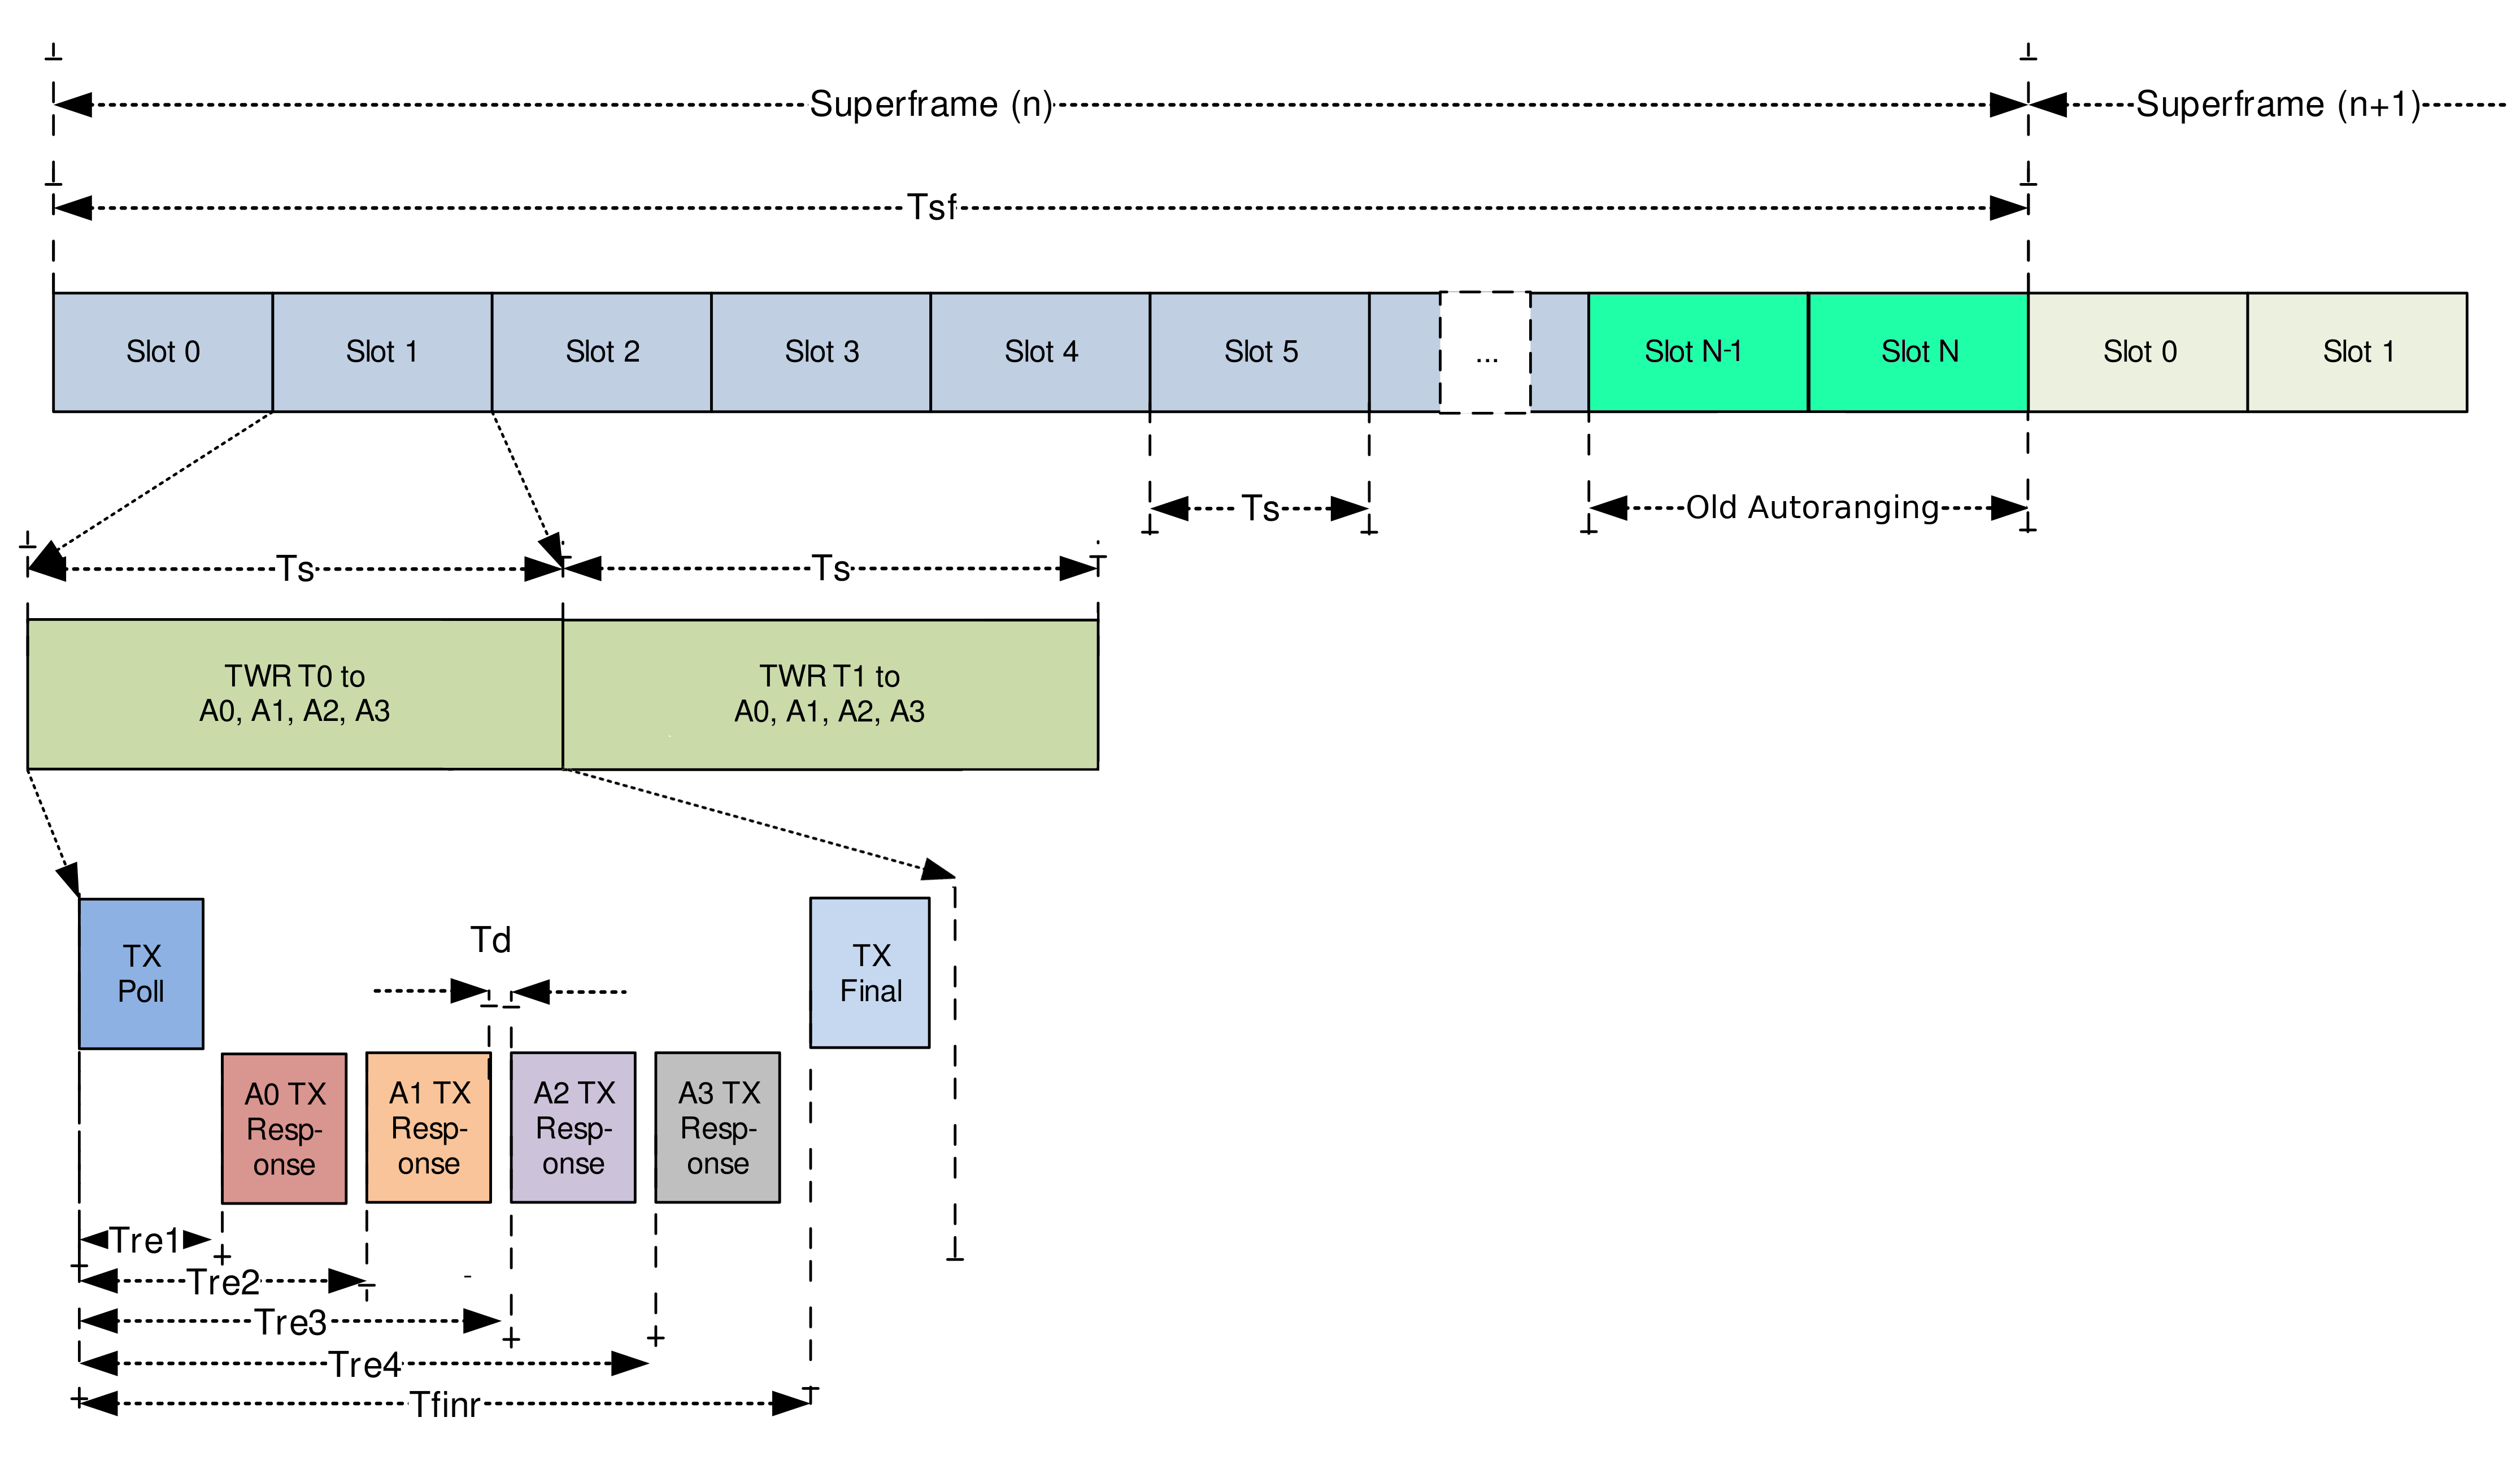
\includegraphics[width=\linewidth]{frame_superframe_a2a.png}
\end{frame}

\begin{frame}[shrink=10, label={anchors_responses_turn}]{Gestione delle risposte delle ancore}
  Come visibile dallo schema riportato nella slide precedente le ancore rispondono una dopo l'altra \alert{a partire
  dall'ancora A0}.\\
  Per far si che tale ordine sia rispettato, ogni ancora, dopo aver ricevuto il messaggio di Poll, sta in ascolto
  delle risposte di tutte le altre ancore. Nel caso ideale in cui tutte le ancore rispondano, l'ancora i-esima
  invia la sua riposta quando la seguente condizione viene verificata
  \[
  N + I = M
  \]
  dove $N$ rappresenta il numero di risposte che l'ancora i-esima si aspetta ancora di ricevere,
  $I$ è l'ID dell'ancora (nel caso di $4$ ancore l'ID è un intero compreso tra $0$ e $3$) ed $M$
  è il numero totale di risposte che l'ancora attende.\\
  Nel caso in cui una delle risposte non arrivi il sistema prevede un \alert{meccanismo di timeout} che consente
  all'ancora i-esima di inviare comunque la risposta nel momento giusto.
\end{frame}

\begin{frame}{Gestione di più tag}
  Al fine di rendere effettivo il protocollo di trasmissione a divisione di tempi, nel caso di più tag,
  l'ancora A0 ricopre un ruolo di arbitraggio. In particolare corregge i tempi di attivazione
  di ogni tag come spiegato di seguito.\\
  Ogni tag invia un messaggio di Poll ogni \alert{activation period} $a_p$
  \[
  a_p = T_{sp} + T_{sr} + T_{sc}
  \]
  \begin{itemize}
  \item[-] $T_{sp}$: periodo ideale di attivazione (detto Sleep Poll) $ = T_{sf}$ : durata del Superframe 
  \item[-] $T_{sr}$: alla prima iterazione vale $\SI{10}{\milli\second}$ successivamente vale  $\SI{0}{\milli\second}$
    (detto Sleep Random)
  \item[-] $T_{sc}$: correzione calcolata dall'\alert{Ancora 0} ed inviata al \alert{tag i-esimo} (detto Sleep Correction)
    nella risposta
  \end{itemize}
\end{frame}

\begin{frame}{Calcolo della correzione $T_{sc}$}
  La correzione viene calcolata in base ad un errore calcolato come la differenza tra il tempo atteso
  d'arrivo del Poll e quello effettivo (dal punto di vista dell'ancora 0)
  \[
  e = t_{i}^{a} - t_{rx}
  \]
  La correzione vale
  \[
  \begin{cases}
    T_{sc} = e \quad \quad \quad \quad \text{se } e < -\frac{T_{sf}}{2}\\
    T_{sc} = T_{sf} + e \quad \quad \text{altrimenti}
  \end{cases}
  \]
  Di seguito sono riportati degli esempi
\end{frame}

\begin{frame}{Calcolo Calcolo del tempo di attivazione $T_{sc} = e$}
  Nel seguente esempio si considera il caso $e < -\frac{T_{sf}}{2}$.\\
  Il tempo di riattivazione del tag $t_{i+1}^{t}$ è:
  \[
  t_{i+1}^{t} = t_{i}^{t} + T_{sf} + T_{sc} = t_i^a - (\cancel{e} + Tof) + T_{sf} + \cancel{e} = t_i^a - Tof + T_{sf} 
  \]
  \begin{center}
    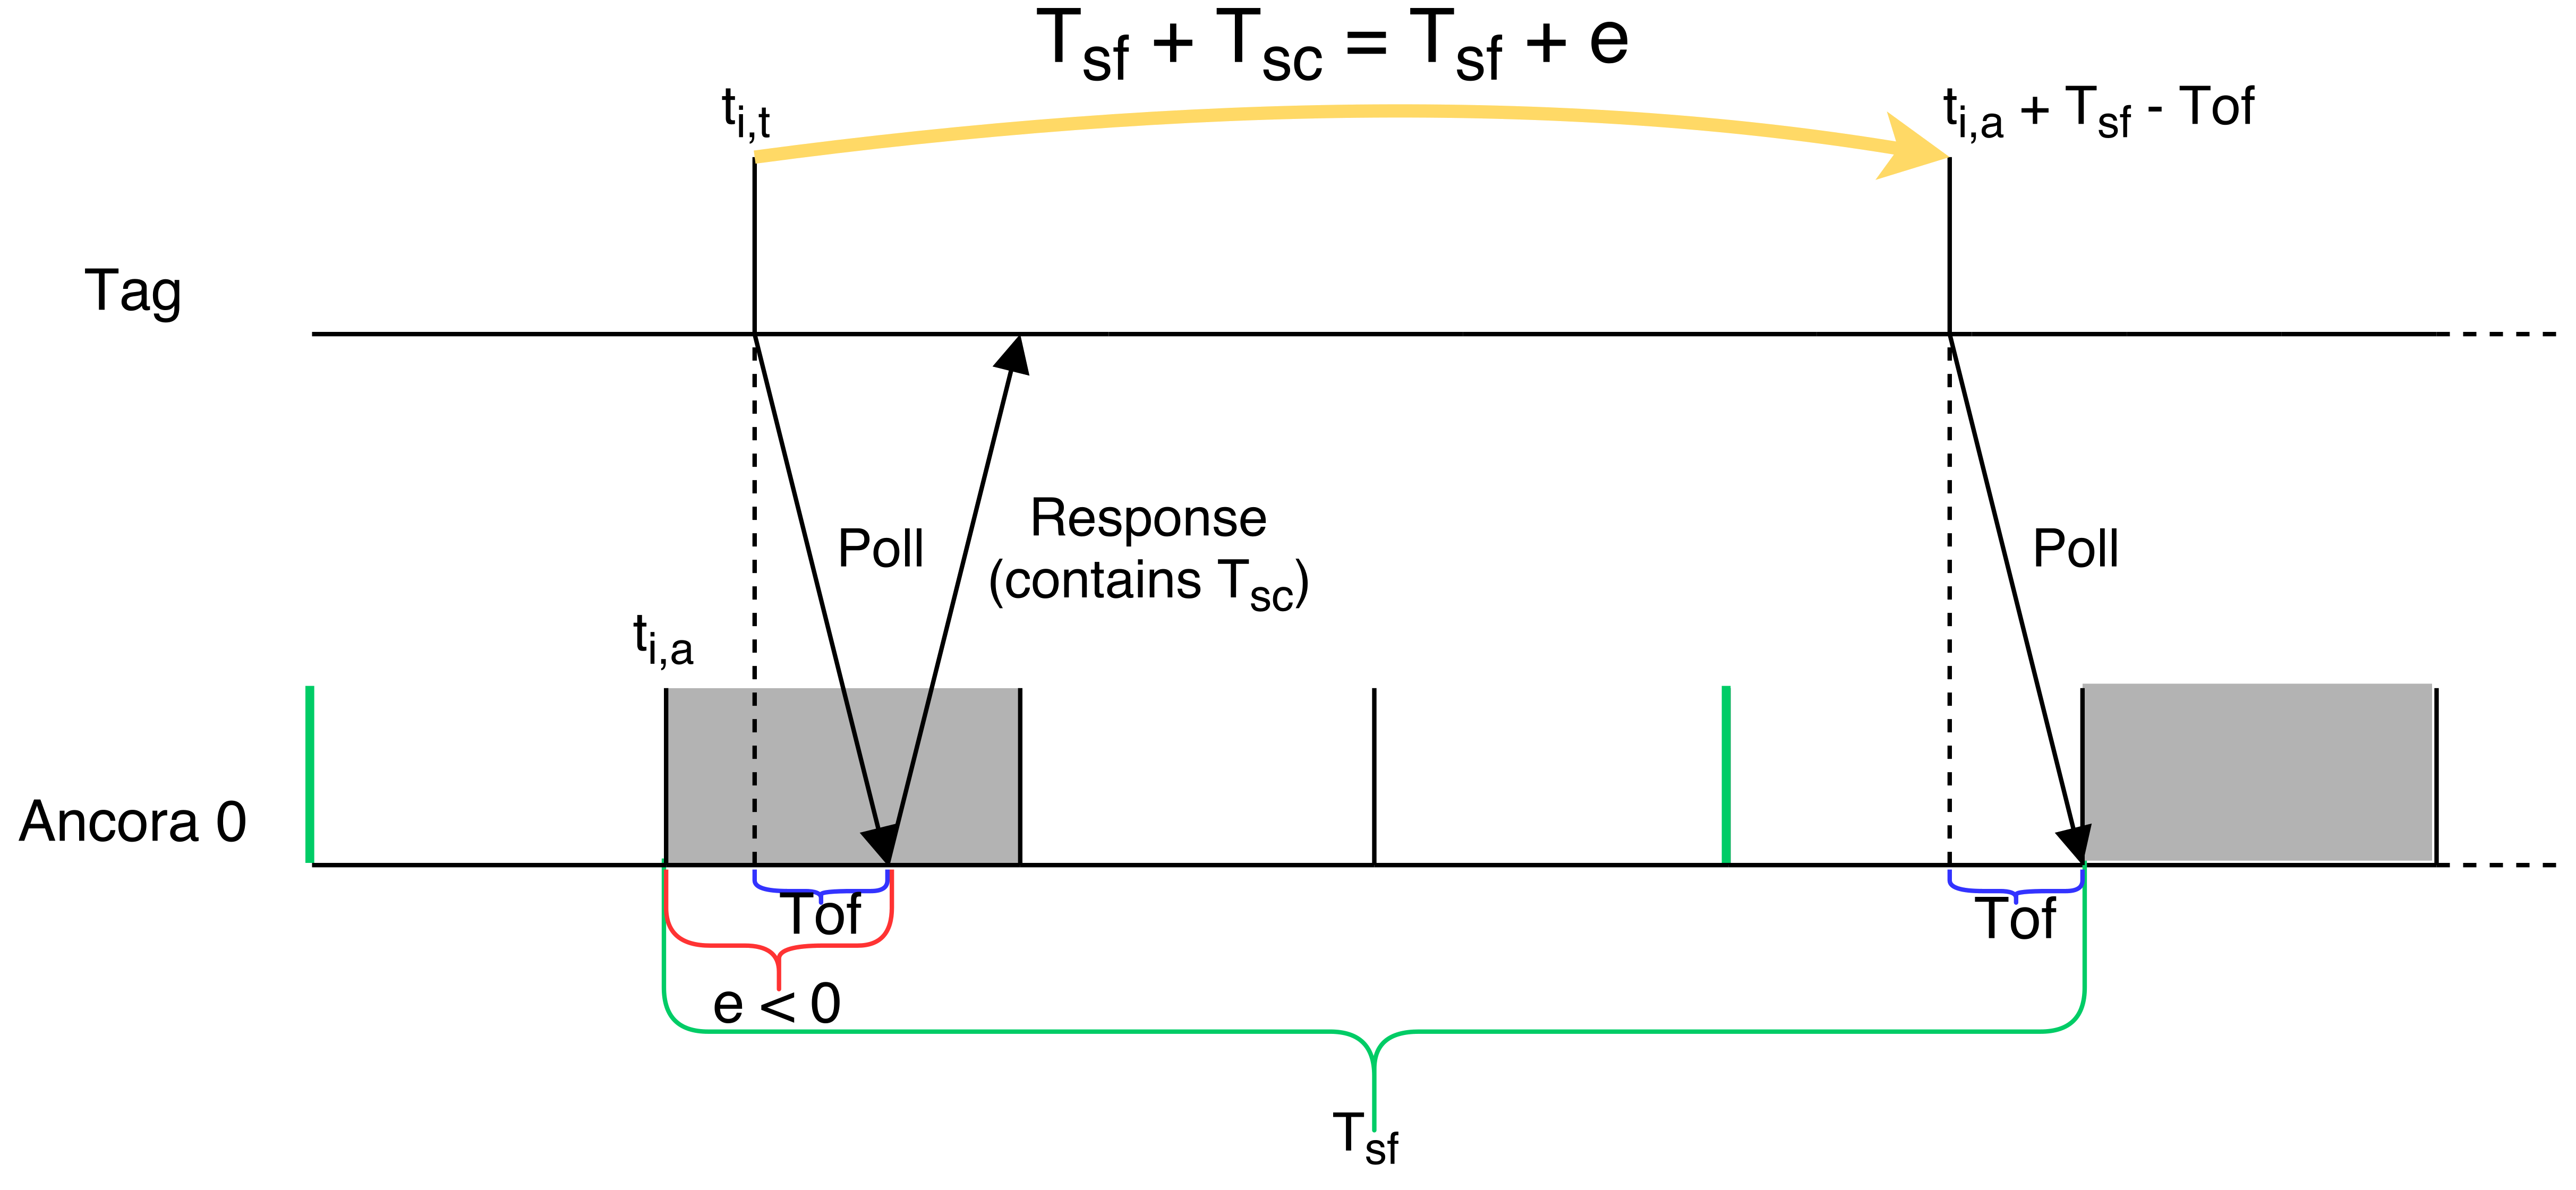
\includegraphics[width=\linewidth]{sleep_correction_less_half_superframe.png}
  \end{center}
\end{frame}

\begin{frame}{Calcolo del tempo di attivazione $T_{sc} = e + T_{sf}$}
  Nel seguente esempio si considera il caso $-\frac{T_{sf}}{2}$ \le e < 0$.\\
  Il tempo di riattivazione del tag $t_{i+1}^{t}$ è:
  \[
  t_{i+1}^{t} = t_{i}^{t} + T_{sf} + T_{sc} = t_i^a - (\cancel{e} + Tof) + T_{sf} + (\cancel{e} + T_{sf}) = t_i^a - Tof + 2T_{sf} 
  \]
  \begin{center}
    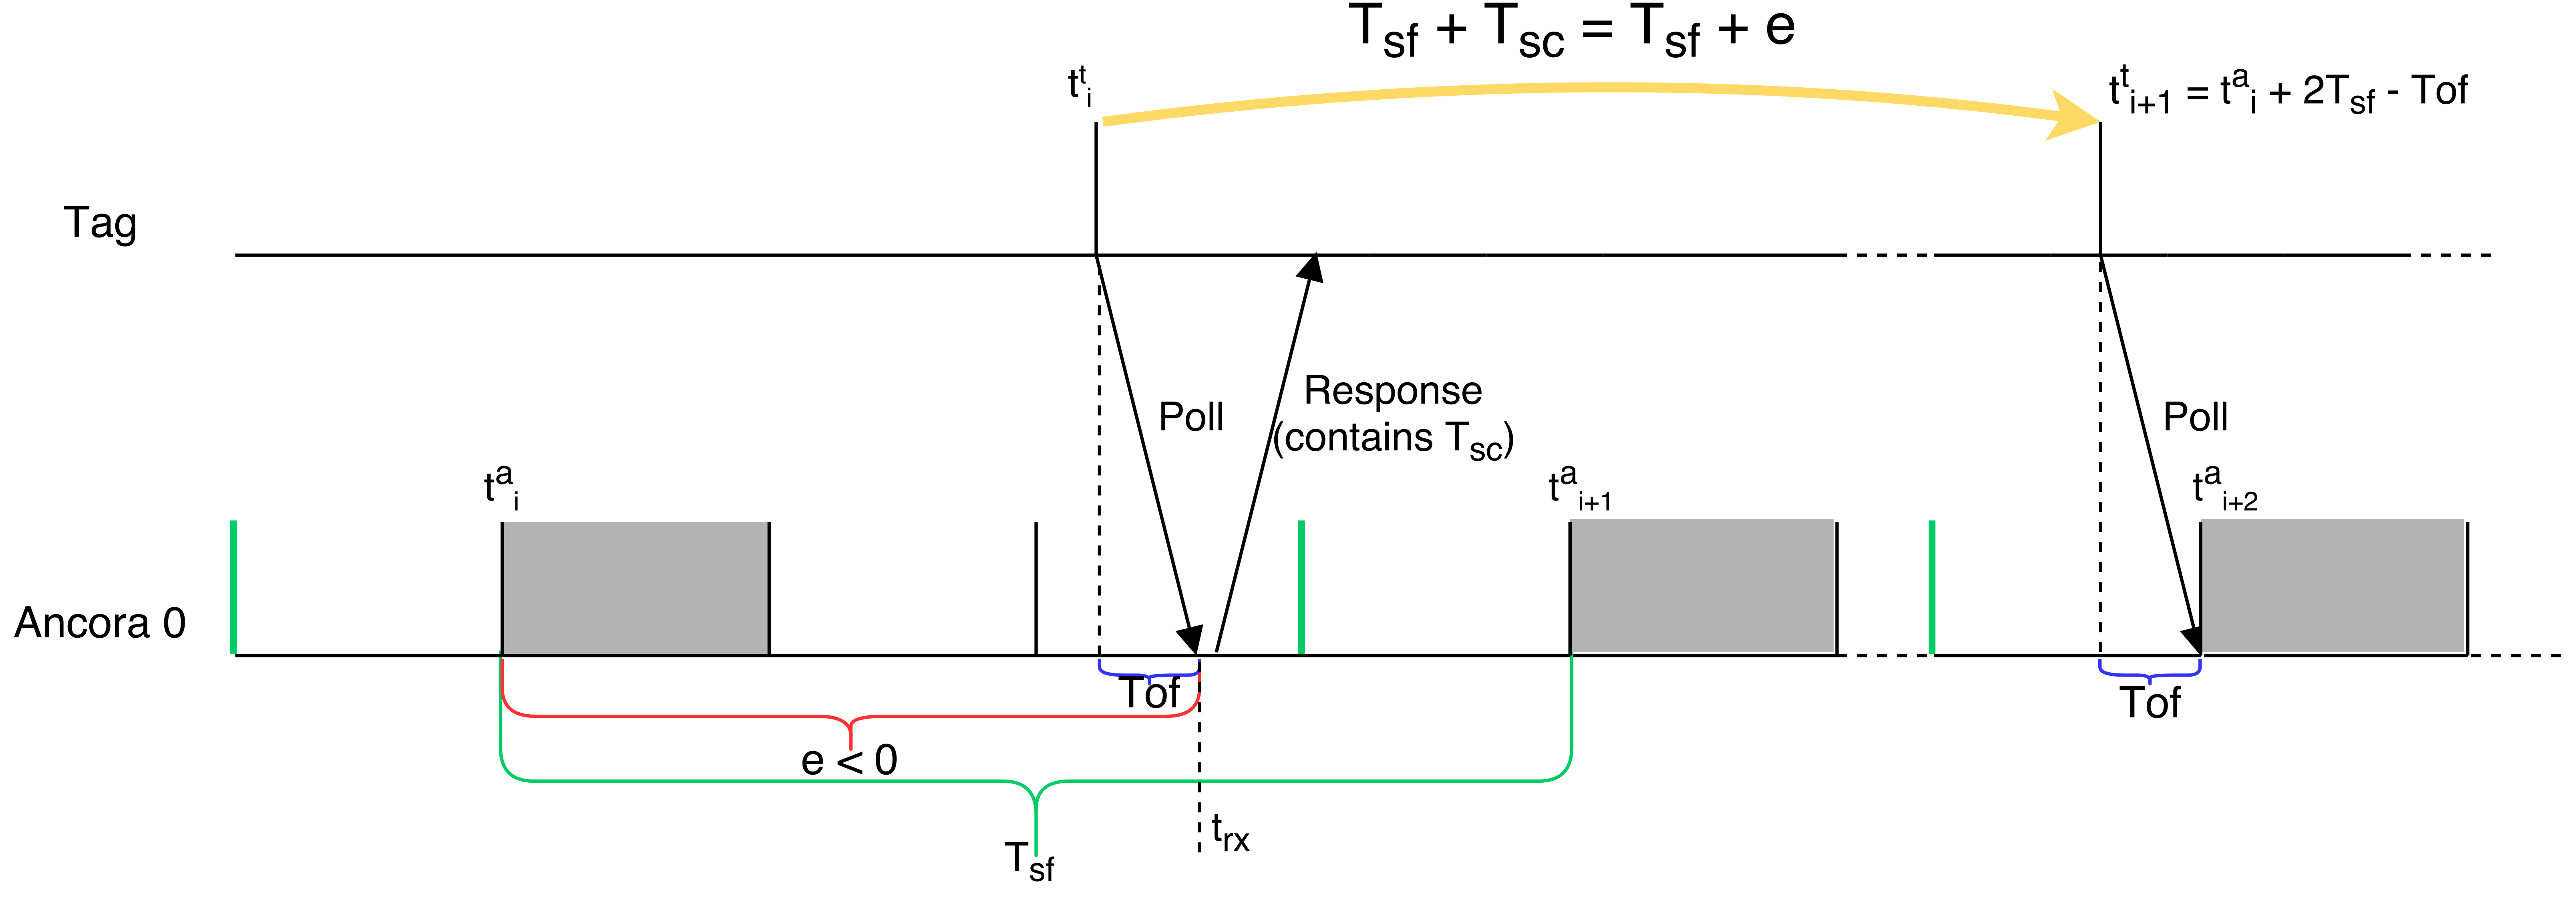
\includegraphics[width=\linewidth]{sleep_correction_greater_half_superframe.png}
  \end{center}
\end{frame}

\begin{frame}{Contributo di Pinna, Malagoli e Giannini}
  Dopo aver chiarito la struttura di frame e superframe è possibile comprendere
  il contributo degli studenti Pinna, Malagoli e Giannini.\\
  Al fine di aumentare la frequenza di ranging è stata ridotta la durata del superframe
  a quella di un solo frame.
  \begin{center}
    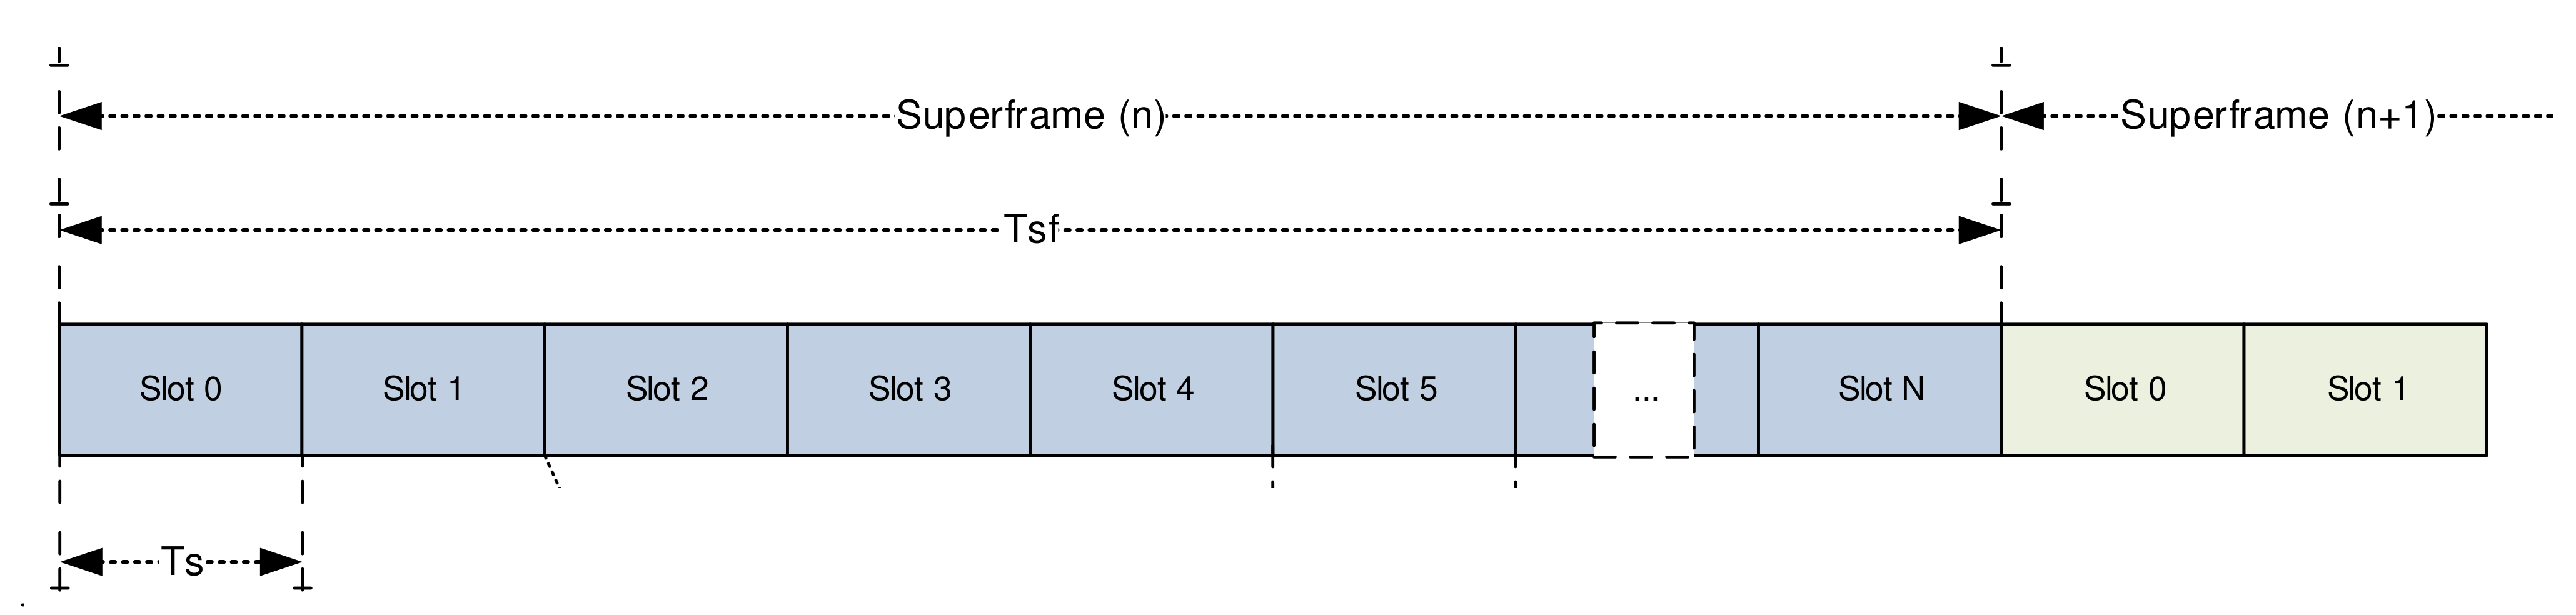
\includegraphics[width=\linewidth]{pmg_frames_removal.png}
  \end{center}
  In questa configurazione
  \begin{itemize}
  \item[-] il sistema è utilizzabile con un solo tag;
  \item[-] il tempo di superframe è $T_{sf} = T_s = \SI{10}{\milli\second}$;
  \item[-] la frequenza è $ f = \SI{100}{\hertz}$.
  \end{itemize}
\end{frame}


\section{Descrizione procedura di Autoranging presente nel Firmware}

\begin{frame}{Modalità di Autoranging inclusa nel Firmware}  
  \begin{center}
    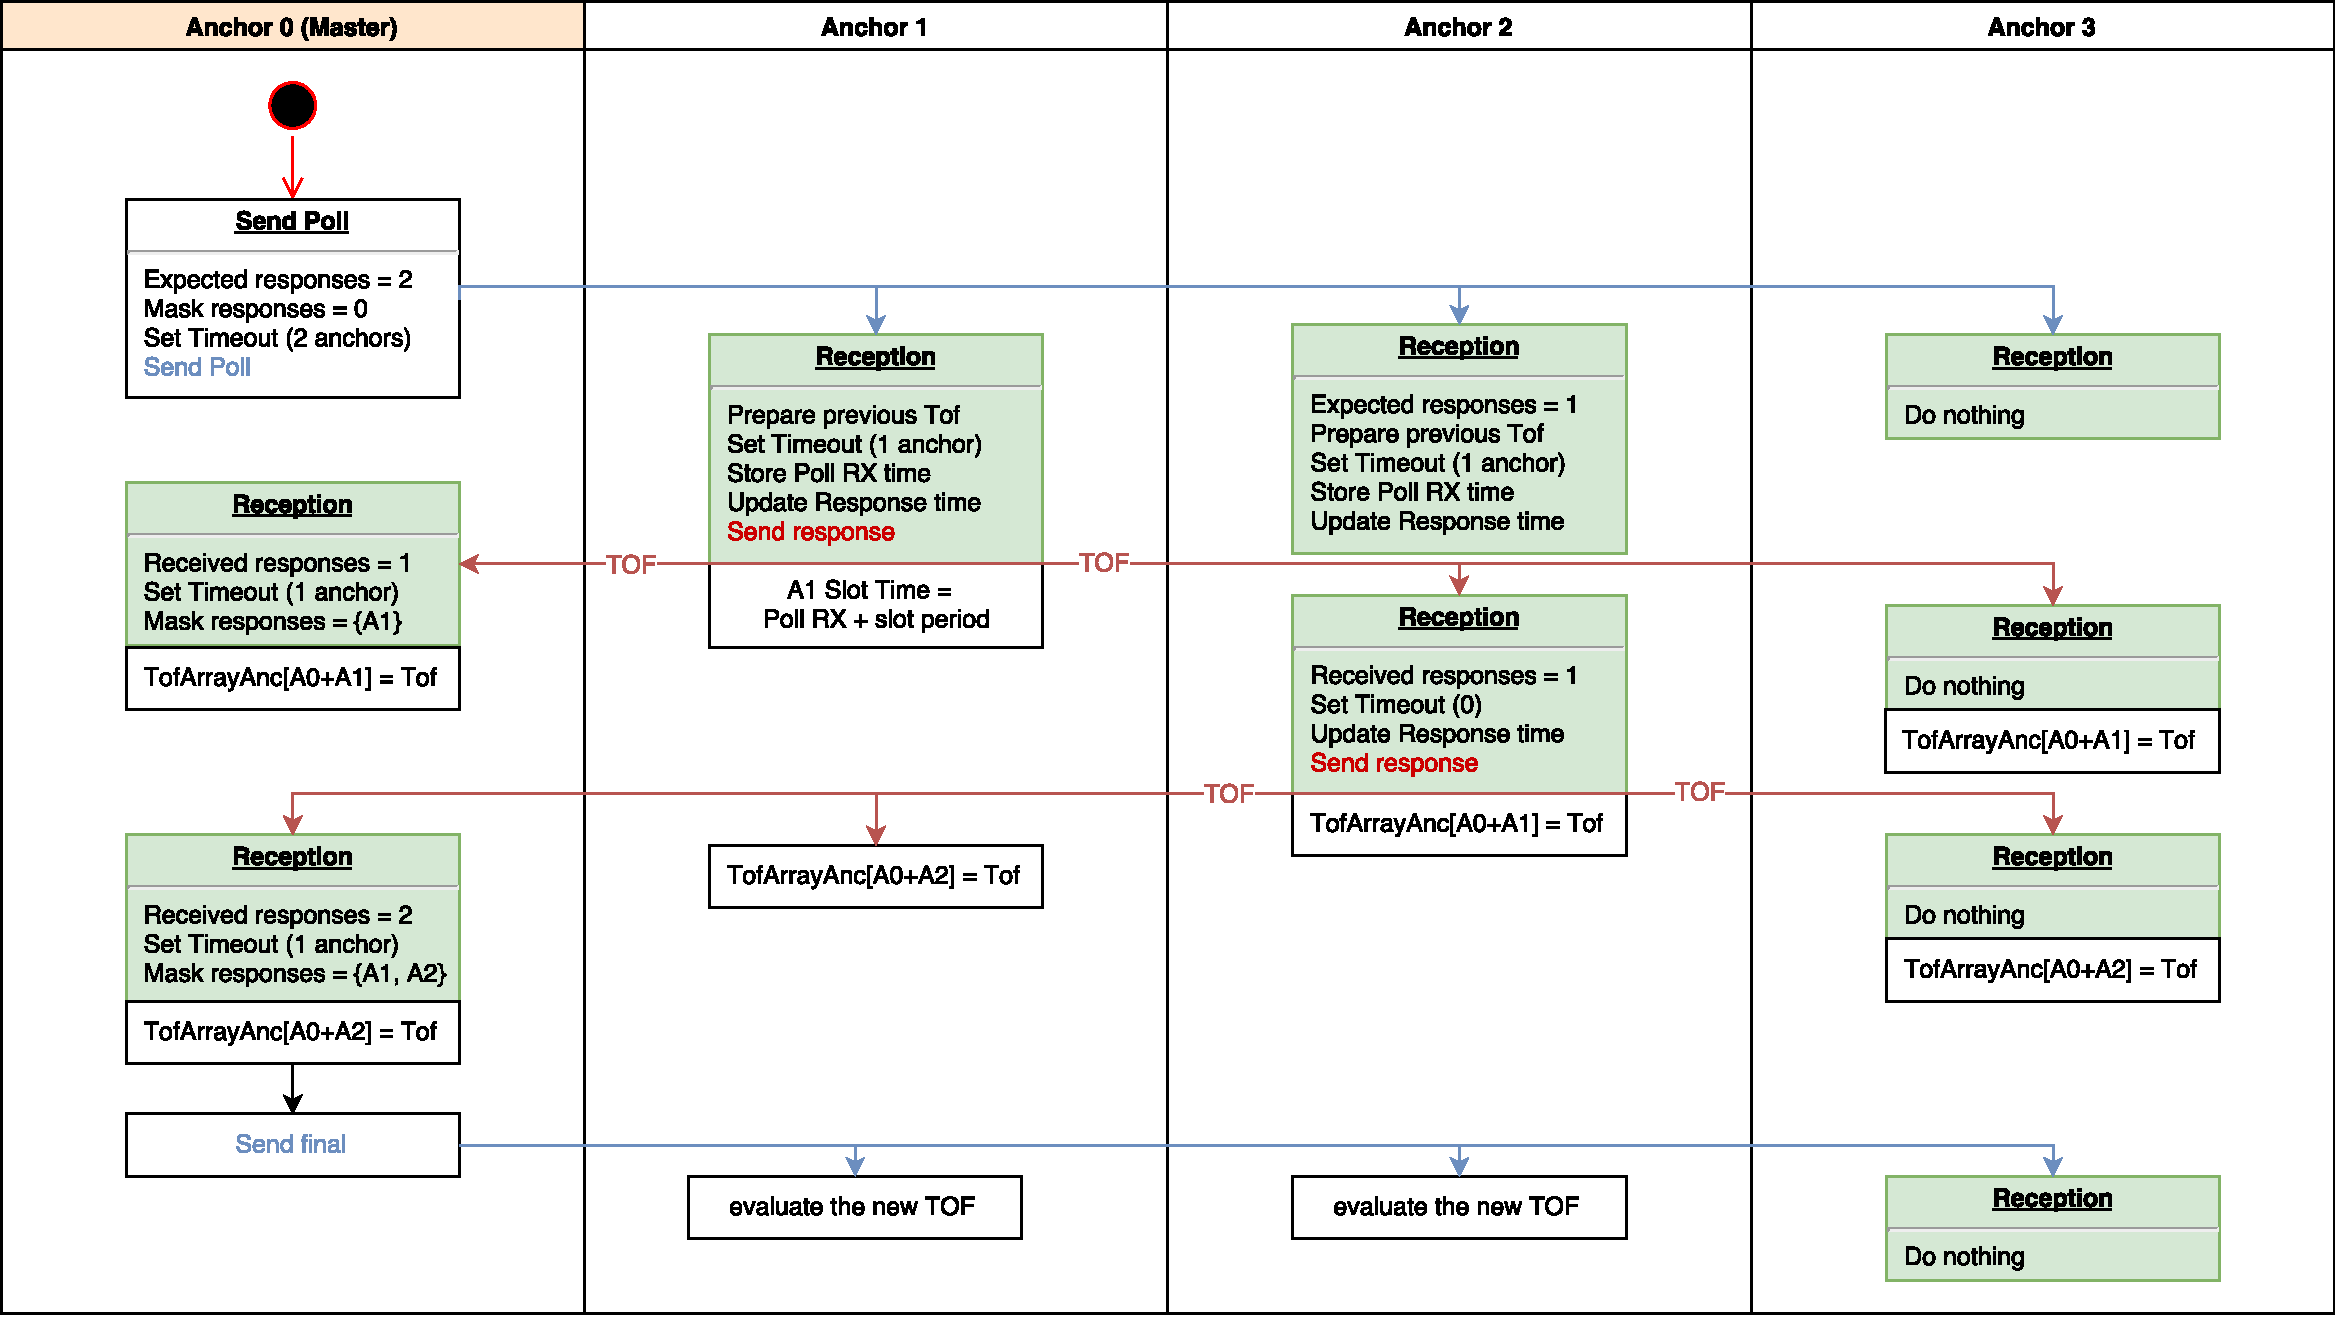
\includegraphics[width=\linewidth]{A2A_oldA0.pdf}
  \end{center}
\end{frame}

\begin{frame}{Modalità di Autoranging inclusa nel Firmware}
  \begin{center}
    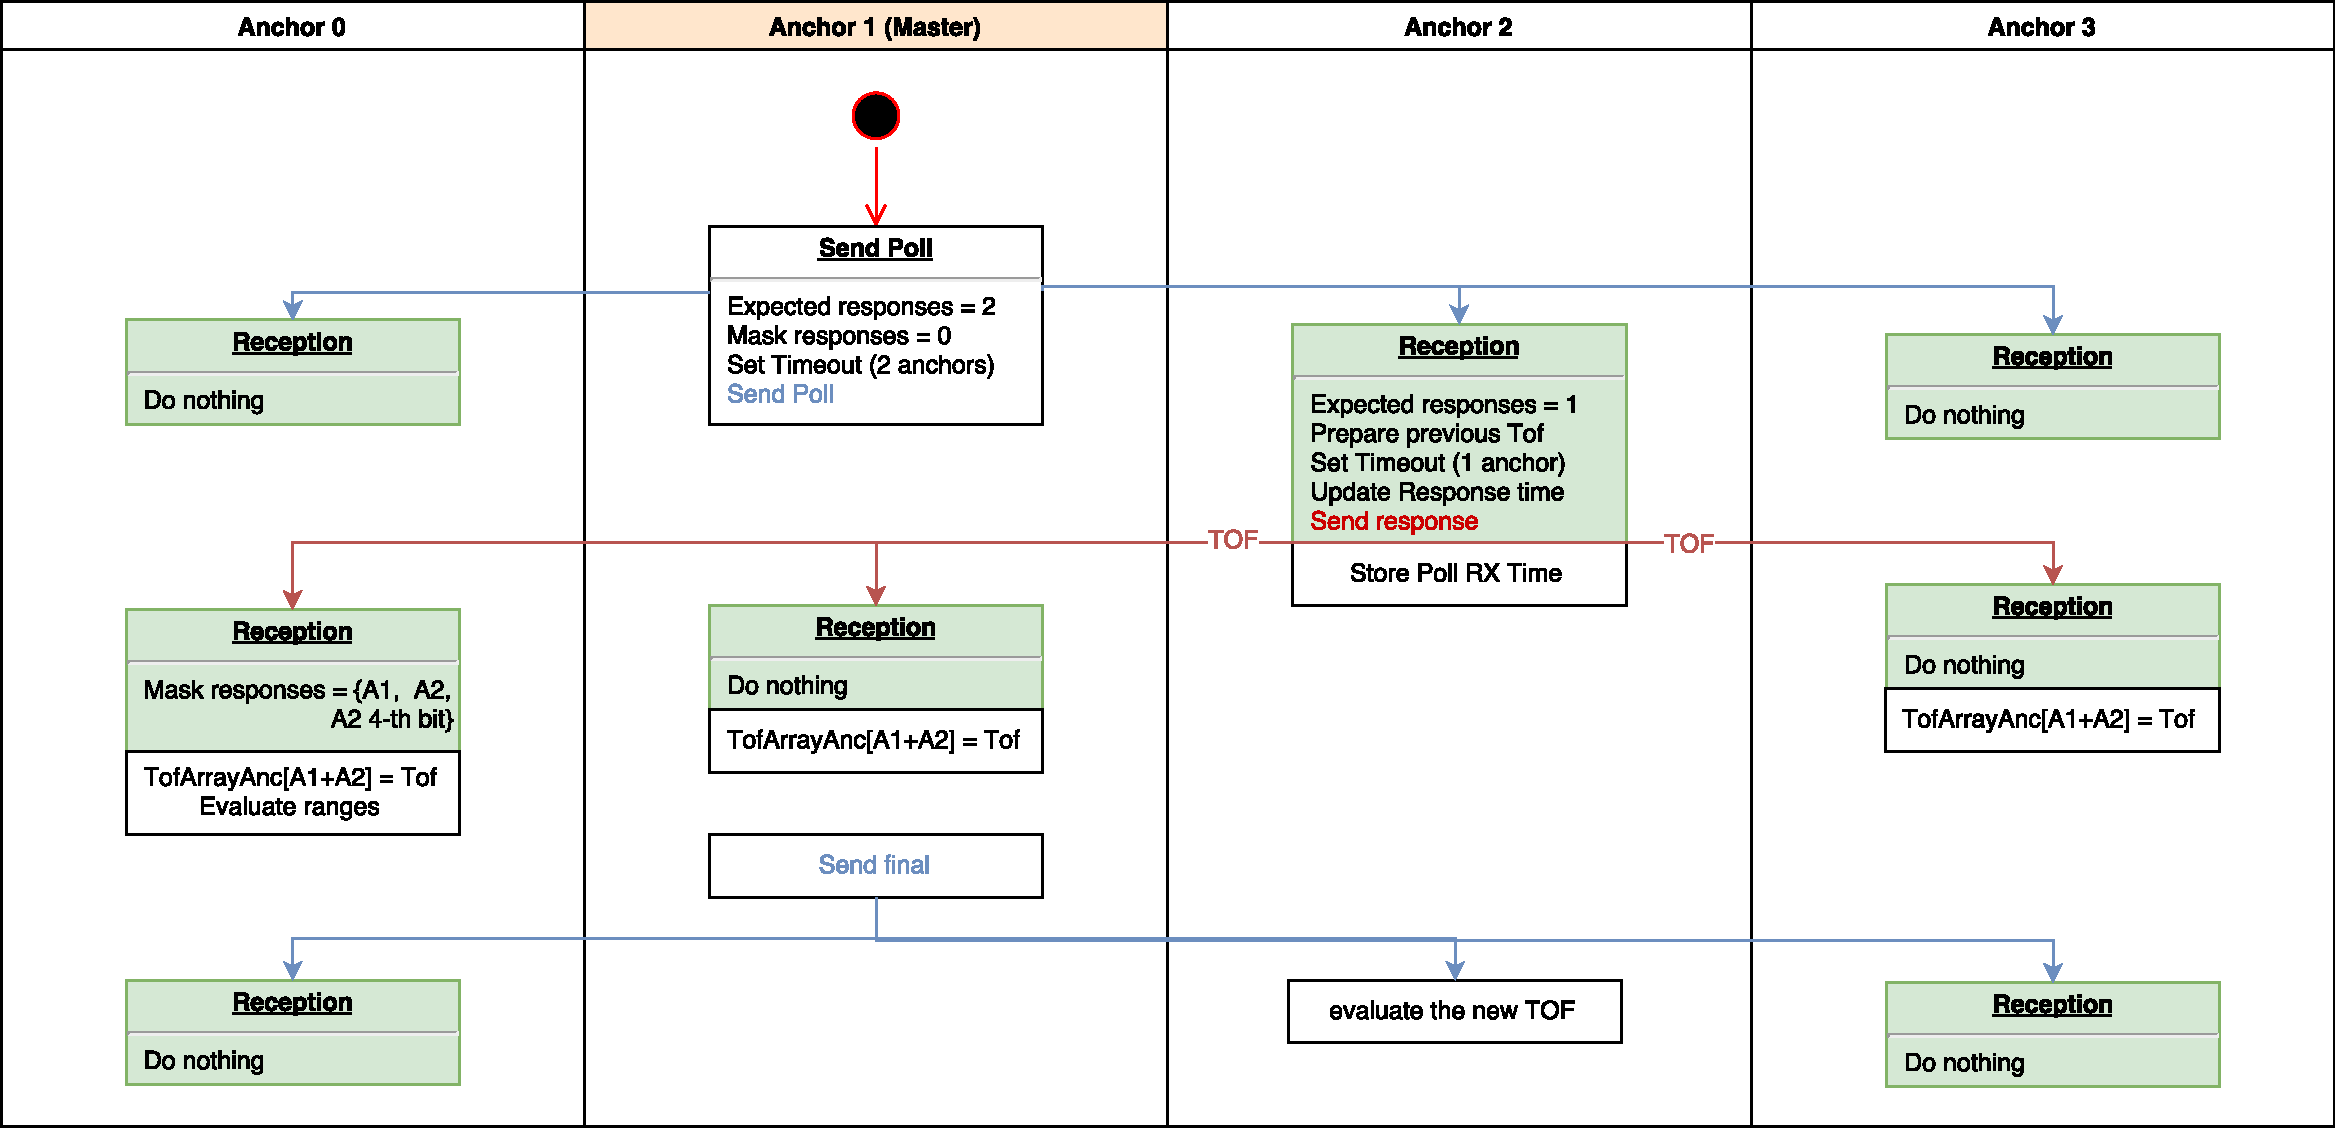
\includegraphics[width=\linewidth]{A2A_oldA1.pdf}
  \end{center}
\end{frame}

\begin{frame}{Considerazioni}
  La procedura di autoranging presente nel firmware:
  \begin{itemize}
  \item [-] calcola solo 3 su 6 dei range richiesti per valutare la posizione delle ancore;
  \item [-] non spedisce i range calcolati / la loro media al tag;
  \item [-] è implementata mediante parti di codice specifiche per ogni ancora quindi \alert{non}
    facilmente estensibile al caso di più ancore;
  \item [-] a parita di scelta del superframe period e dello slot period \alert{riduce} di $N$ il numero
    massimo di tag utilizzabili poiché la procedura avviene negli ultimi $N$\footnote{nel caso del
      firmware $N = 2$} slot.
  \end{itemize}
\end{frame}

\section{Nuova procedura di autoranging}

\begin{frame}{Nuova procedura di autoranging}
  A differenza della procedura originale la nuova procedura \alert{non} avviene durante la fase
  di ranging portata avanti dal tag ma avviene in una fase preliminare durante la quale il tag sta in
  attesa.
  \par
  L'intera procedura si divide in 3 parti. Ogni ancora \alert{a turno}: 
  \begin{itemize}
  \item [1.] valuta $M$ volte i range di interesse, i.e. l'ancora
    j-esima raccoglie i range $r_{j,j+1}$ ... $r_{j,N-1}$ con $N$ il numero di ancore e $j<N$;
  \item [2.] calcola la media dei range raccolti;
  \item [3.] invia i range medi al tag ogni volta che risponde ad un suo Poll.
  \end{itemize}
\end{frame}

\begin{frame}{Simmetria}
  In linea di principio quando l'ancora j-esima esegua la sua fase di raccolta dei range non sarebbe
  necessario che le ancore con indice $i < j$ partecipino alla procedura poiché sono di interesse solo
  i range $r_{j,k}$ con $j < k < N$. Tuttavia facendo partecipare sempre tutte le ancore è possibile
  raccogliere per $M$ volte ciascun range eseguendo $M/2$ istanze di range per ogni ancora invece che $M$.

  \begin{exampleblock}{Numero di istanze di range richieste}
    Date $N$ ancore per raccogliere $M$ volte ciascun range di interesse sono richieste
    \[
    N \frac{M}{2}
    \]
    istanze di ranging
  \end{exampleblock}
\end{frame}

\begin{frame}{Simmetria - esempio}
  Sia $i<j$, l'ancora $A_i$ esegue $M/2$ istanze di ranging
  \begin{center}
    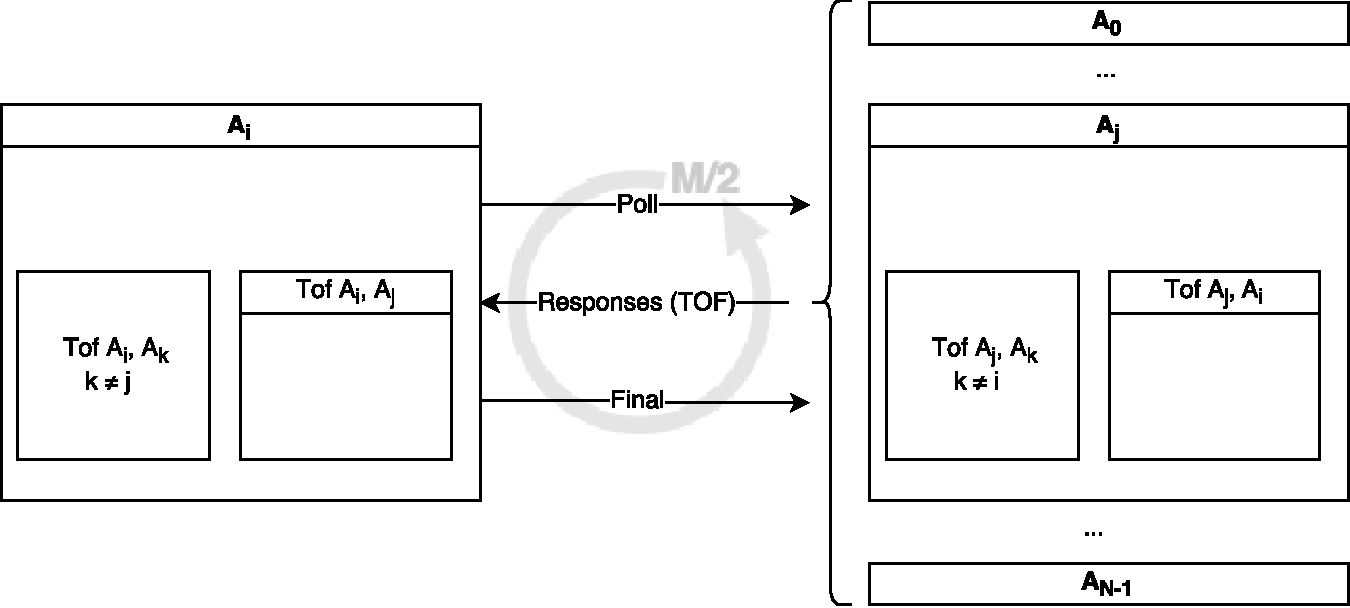
\includegraphics[width=\linewidth]{new_autoranging_1.pdf}
  \end{center}
\end{frame}

\begin{frame}{Simmetria - esempio}
  L'ancora $A_i$ ha memorizzato $M/2$ misure di ranging
  \begin{center}
    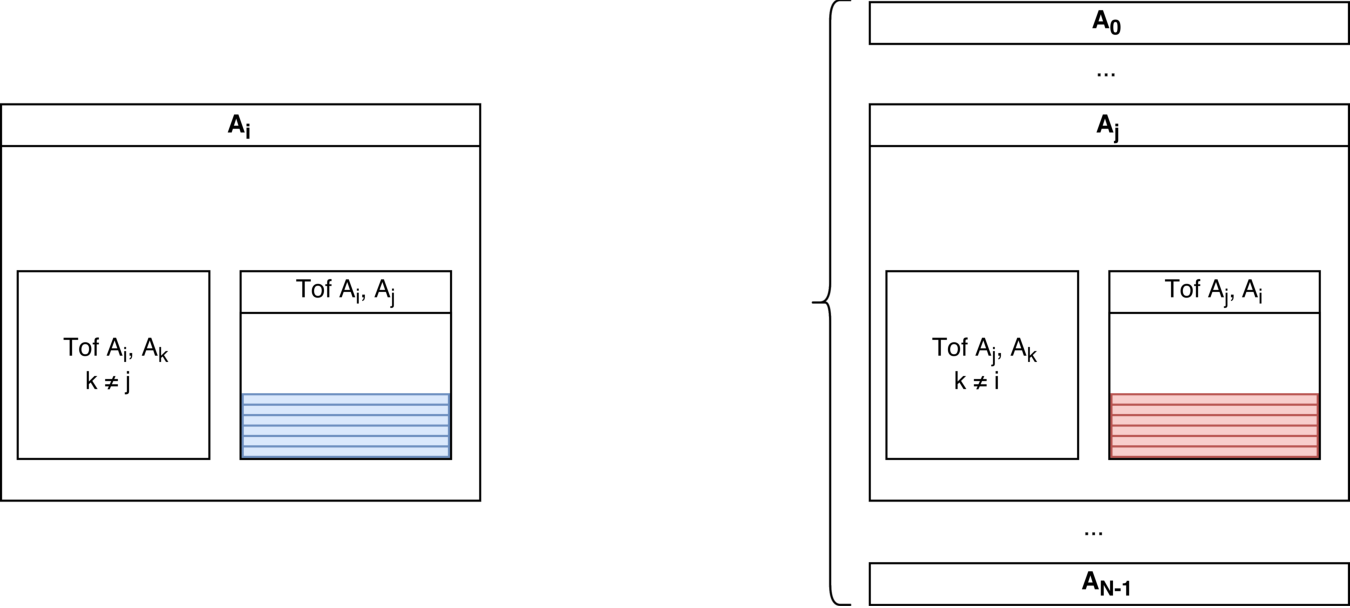
\includegraphics[width=\linewidth]{new_autoranging_2.pdf}
  \end{center}
\end{frame}

\begin{frame}{Simmetria - esempio}
  Successivamente l'ancora $A_j$ esegue $M/2$ istanze di ranging
  \begin{center}
    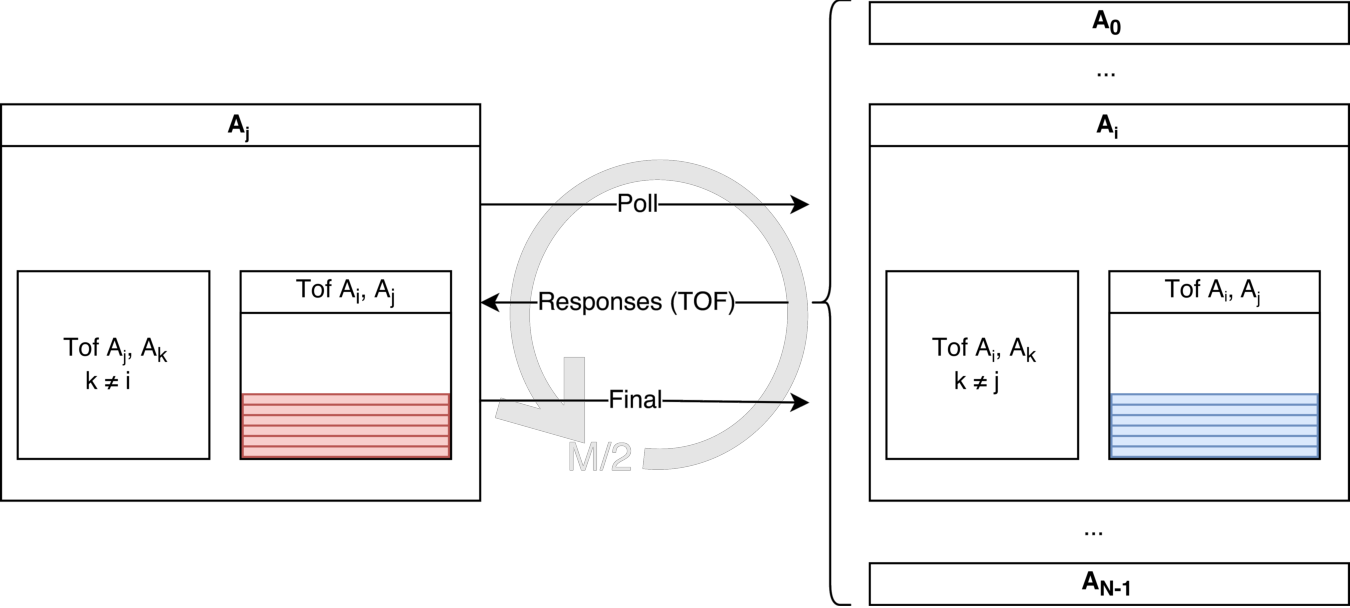
\includegraphics[width=\linewidth]{new_autoranging_3.pdf}
  \end{center}
\end{frame}

\begin{frame}{Simmetria - esempio}
  L'ancora $A_i$ colleziona ulteriori $M/2$ misure
  \begin{center}
    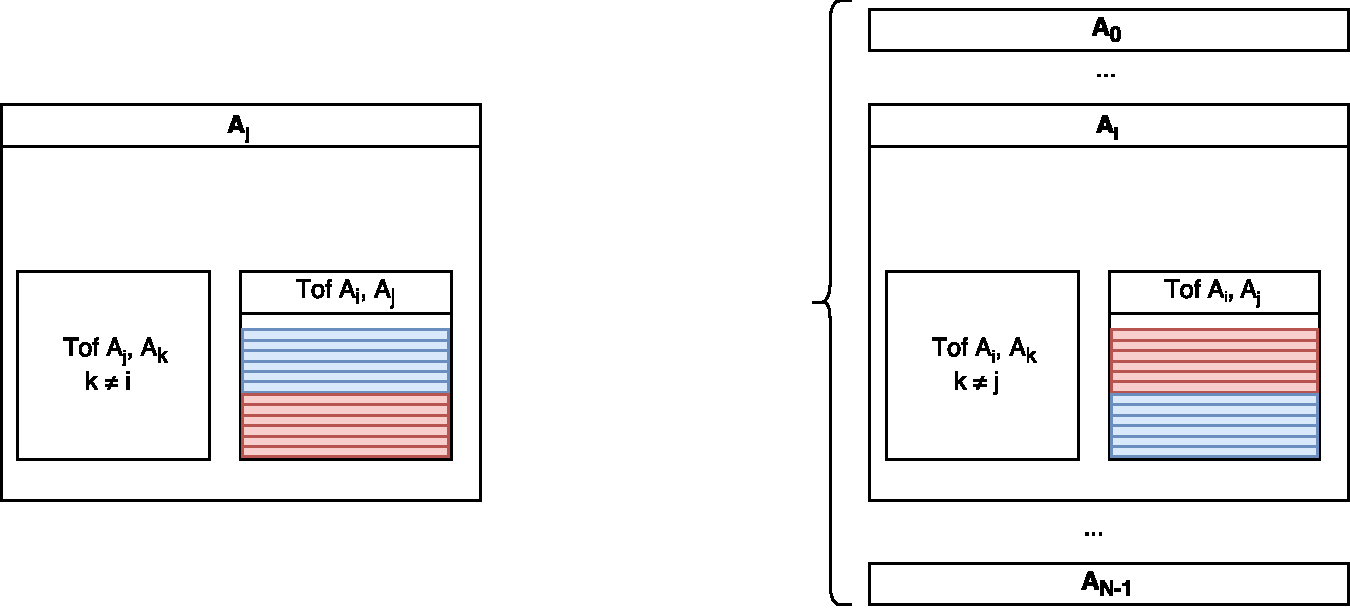
\includegraphics[width=\linewidth]{new_autoranging_4.pdf}
  \end{center}
\end{frame}

\begin{frame}{Simmetria - esempio}
  Le distribuzioni delle misure raccolte sfruttando la simmetria sono simili 
  \begin{center}
    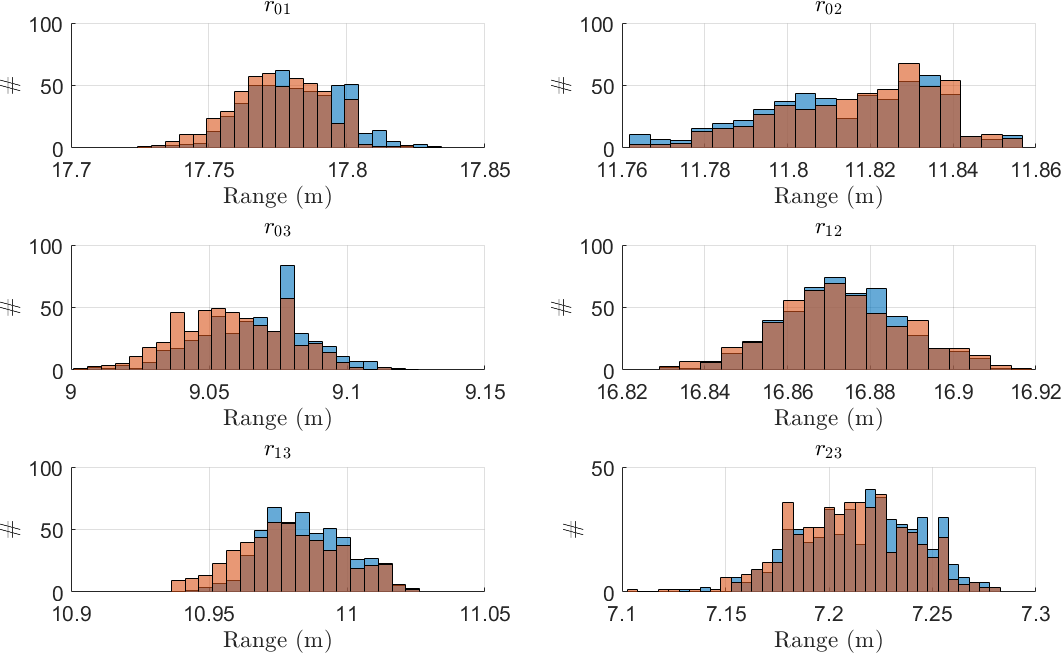
\includegraphics[scale=0.37]{autoranging.png}
  \end{center}
\end{frame}

\section{Guida al codice sviluppato}
\begin{frame}{File modifica e file nuovi}
  \begin{columns}
    \begin{column}{0.7\textwidth}
      Per implementare la \alert{nuova} procedura di autoranging
      è stato necessario inervenire sul codice.\\
      In \textcolor{red}{rosso} sono indicati i file modificati e in
      \textcolor{violet}{viola} i nuovi file prodotti.
    \end{column}
    \begin{column}{0.3\textwidth}
      \centering
      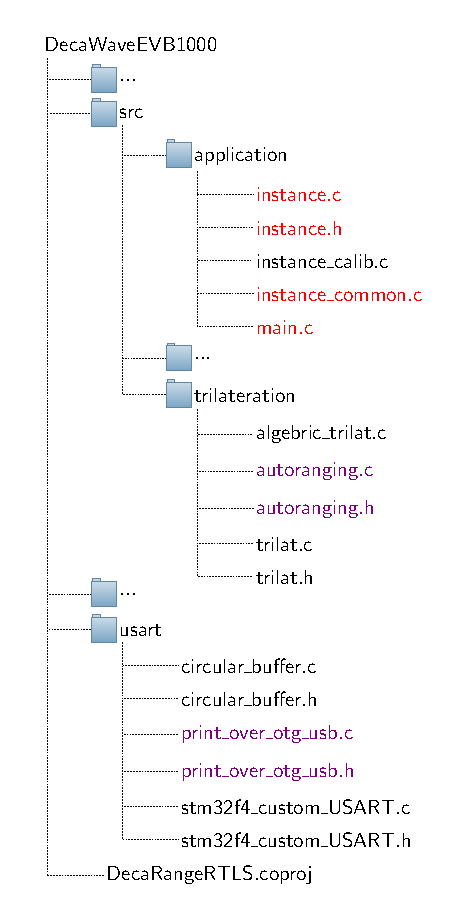
\includegraphics[height=20em]{file_tree.pdf}
    \end{column}
  \end{columns}

\end{frame}

\section{Header instance.h}
\begin{frame}[fragile, shrink=10]{Header instance.h - Define}
  Sono state aggiunte le seguenti define nel file instance.h

  \begin{block}{\lstinline[language=C]!#define NUM_AUTORNG_RNG M/2!}
  Definisce il numero $M$ di misure raccolte durante l'autoranging da ogni ancora master per ogni range di interesse.\\
  \textcolor{dgreen}{esempio:} A0 raccoglie $M$ misure di $r_{01}$, $M$ misure di $r_{02}$ ed $M$ misure di $r_{03}$.
  \end{block}

  \begin{block}{\lstinline[language=C]!#define AUTORANGING_MAX_TIMEOUT_TAG ...!}
  Tempo in \SI{}{\milli\second} dopo il quale il tag inizia la normale procedura di ranging se non
  riceve più messaggi di POLL inviati da un'ancora master.
  \end{block}

  \begin{block}{\lstinline[language=C]!#define  ANCH_FINAL_MSG_LEN 34!}
    Lunghezza del messaggio di tipo \lstinline[language=C]!RTLS_DEMO_MSG_ANCH_FINAL!.\\
    Essa è pari a quella del messaggio di tipo \lstinline[language=C]!RTLS_DEMO_MSG_TAG_FINAL! più uno dato
    che contiene un byte in più che serve ad indicare alle ancore che l'autoranging per la corrente
    ancora master è terminato.
  \end{block}
\end{frame}

\begin{frame}[fragile]{Header instance.h - Define}
  \begin{block}{\lstinline[language=C]!#define NUM_ALL_AUTORANING_RANGES!}
  Numero complessivo di range che il tag si aspetta di ricevere da tutte le ancore.\\
  Scritto in funzione del numero totale di ancore $N$.\\
  \textcolor{dgreen}{esempio:} per $4$ ancore
  \[
  |\{r_{01}, r_{02}, r_{03}, r_{12}, r_{13}, r_{23}\}| = 3 + 2 + 1 = 6
  \]
  \alert{in generale:}
  \[
  \frac{(N-1) (N-1+1)}{2} = \frac{(N-1)N}{2}
  \]
  \end{block}
\end{frame}

\begin{frame}[fragile]{Header instance.h - Define}
  \begin{block}{\lstinline[language=C]!#define END_AUTORANGING 33!}
    Posizione, all'interno di \lstinline[language=C]!instance_data[0].msg_f.messageData!, del byte
    che indica la fine della procedura di autoranging per una data ancora master.\\
    In questo caso messageData contiene un messaggio di tipo \lstinline[language=C]!RTLS_DEMO_MSG_ANCH_FINAL!.
  \end{block}
  \begin{block}{\lstinline[language=C]!#define AUTORANGING_RANGES 8!}
    Posizione, all'interno di \lstinline[language=C]!instance_data[0].msg_f.messageData!, a partire dalla quale
    l'ancora inserisce le medie dei range che le competono.\\
    In questo caso messageData contiene un messaggio di tipo \lstinline[language=C]!RTLS_DEMO_MSG_ANCH_RESP!.
  \end{block}
\end{frame}

\begin{frame}[fragile]{Header instance.h - Struct \lstinline[language=C]!sfConfig_t!}
  Le seguenti \lstinline[language=C]!struct! sono state modificate
  \begin{C}
    typedef struct
    {
      ...
      uint16 tagPollSleepDly;
      uint16 anchPollSleepDly;
      ...
    } sfConfig_t;
  \end{C}
  È stato aggiunto il campo \lstinline[language=C]!anchPollSleepDly! e il campo \lstinline[language=C]!pollSleepDly! è stato rinominato
  \lstinline[language=C]!tagPollSleepDly! per maggiore chiarezza.\\
  Il campo \lstinline[language=C]!anchPollSleepDly! rappresenta il periodo in \SI{}{\milli\second} di trasmissione dei Poll
  dell'ancora master.

\end{frame}

\begin{frame}[fragile]{Header instance.h - Struct \lstinline[language=C]!instance_data_t!}
  \begin{C}
    typedef struct
    {
      ...
    } instance_data_t;
  \end{C}
  Sono stati aggiunti i seguenti campi
  \begin{block}{\lstinline[language=C]!int32 anchSleepTime_ms!}
    Periodo in \SI{}{\milli\second} di trasmissione dei Poll dell'ancora master
  \end{block}
  
  \begin{block}{\lstinline[language=C]!unsigned long autoranging_poll_time!}
    Se il dispositivo si comporta come ancora in modalità \lstinline[language=C]!ANCHOR_RNG! ed è l'ancora master
    rappresenta l'istante di tempo, secondo l'orologio interno, in cui è stato spedito l'ultimo Poll.\\
    Utilizzato per capire se sono passati \lstinline[language=C]!anchSleepTime_ms! \SI{}{\milli\second} dall'invio dell'ultimo Poll.
  \end{block}
\end{frame}

\begin{frame}{Header instance.h - Struct \lstinline[language=C]!instance_data_t!}
  \begin{block}{\lstinline[language=C]!unsigned long autoranging_poll_time! - continuazione}
    Se invece il dispositivo si comporta come tag in modalità \lstinline[language=C]!TAG_WAIT! rappresenta l'istante di tempo, secondo l'orologio
    interno, in cui il tag ha ricevuto l'ultimo Poll inviato da un'ancora master.\\
    Utilizzato per capire se sono passati \lstinline[language=C]!AUTORANGING_MAX_TIMEOUT_TAG! \SI{}{\milli\second} dalla ricezione
    dell'ultimo Poll inviato da un'ancora master.
  \end{block}
  \begin{block}{\lstinline[language=C]!uint8 autoranging_timeout!}
    Abilitazione del timer usato da un'ancora master per inviare periodicamente Poll alle altre ancore.\\
    Abilitazione del timer usato da un tag in modalità \lstinline[language=C]!TAG_WAIT! per attendere la fine della
    procedura di autoranging.
  \end{block}
\end{frame}

\begin{frame}{Header instance.h - Struct \lstinline[language=C]!instance_data_t!}
  \begin{block}{\lstinline[language=C]!double anchRngArray[MAX_ANCHOR_LIST_SIZE]!}
    Contiene la somma dei range raccolti da una data ancora.\\
    \textcolor{dgreen}{esempio:} sia l'ancora A1. \lstinline[language=C]!anchrRngArray[0]! contiene la somma dei range $r_{01}$,
    \lstinline[language=C]!anchrRngArray[2]! contiene la somma dei range $r_{12}$ e \lstinline[language=C]!anchrRngArray[3]! contiene la somma dei range $r_{13}$.
  \end{block}
  \begin{block}{\lstinline[language=C]!uint16 anchRngArrayCounter!}
    Contiene il numero di misure raccolte per ciascun range di interesse per una data ancora.\\
    \textcolor{dgreen}{esempio:} sia l'ancora A1. \lstinline[language=C]!anchrRngArrayCounter[0]! contiene il numero di misure del range $r_{01}$,
    \lstinline[language=C]!anchrRngArrayCounter[2]! contiene il numero di misure del range $r_{12}$ e \lstinline[language=C]!anchrRngArrayCounter[3]! contiene il numero di misure del range $r_{13}$.
  \end{block}
\end{frame}

\begin{frame}{Header instance.h - Struct \lstinline[language=C]!instance_data_t!}
  \begin{block}{\lstinline[language=C]!uint8 autoRngRangesRxMask!}
    Bitmask. Il bit i-esimo vale 1 se il tag ha ricevuto \alert{tutte} le medie dei range dall'ancora i-esima.
  \end{block}
  \begin{block}{\lstinline[language=C]!double autoRngRangesArray[NUM_ALL_AUTORANGING_RANGES]!}
    Medie dei range ricevute dal tag.\\
    \textcolor{dgreen}{esempio:} Nel caso di 4 ancore \lstinline[language=C]!autoRngRangesArray[0]! $ = r_{01}$,
    \hdots, \lstinline[language=C]!autoRngRangesArray[5]! $ = r_{23}$.
  \end{block}
  \begin{block}{\lstinline[language=C]!float anchorPositionMatrix[3 * MAX_ANCHOR_LIST_SIZE]!}
    Posizioni cartesiane delle ancore ottenute con apposito algoritmo a partire dalle medie dei range salvate
    in \lstinline[language=C]!autoRngRangesArray!.\\
    \alert{in generale:} \lstinline[language=C]!anchorPositionMatrix[i][j]! contiene la coordinata $i$-esima dell'ancora $j$-esima.
  \end{block}
\end{frame}

\begin{frame}{Header instance.h - Struct \lstinline[language=C]!instance_data_t!}
  \begin{block}{\lstinline[language=C]!uint8 tagPositionsSentToViewer!}
    Contatore utilizzato per inviare ad intervalli regolari la posizione delle ancore sulla porta seriale
    virtuale (USB OTG VCP). Tali posizioni sono utilizzate dal Viewer 3D (di cui si parlerà nel seguito).
  \end{block}
  \begin{block}{\lstinline[language=C]!uint16 anchorRngMaster!}
    Contiene l'ID corrente dell'ancora master durante l'autoranging.
  \end{block}
\end{frame}

\begin{frame}[shrink=10]{Header instance.h - Struct \lstinline[language=C]!instance_data_t! - \lstinline[language=C]!rxResponseMaskAnc!}
  Il campo \lstinline[language=C]!rxResponseMaskAnc! era già presente nella struct \lstinline[language=C]!instance_data_t!.
  \par
  Durante la procedura di autoranging l'ancora master mette ad $1$ il bit i-esimo se ha rivecuto risposta dall'ancora i-esima.
  \par
  Le ancore \alert{non} master, invece, utilizzano questo campo per decidere quando è il momento di rispondere.
  Rispetto alla normale procedura di ranging, nella quale la prima ancora a rispondere è sempre l'ancora A0, durante la
  procedura di autoranging è più complicato, per ogni ancora, decidere quando rispondere. Infatti quando l'ancora master non è A0
  l'ordine in cui le ancore devono rispondere non è scontato. Ad esempio quando A2 si comporta da ancora master l'ordine di risposta delle ancore
  dovrà essere A0, A1, A3.\\
  Per non scrivere un codice ad hoc per specificare l'ordine di risposta al variare di ogni ancora master la maschera \lstinline[language=C]!rxResponseMaskAnc!
  è stata utilizzata come spiegato nell'esempio della slide successiva.
\end{frame}

\begin{frame}[shrink=10]{Header instance.h - Struct \lstinline[language=C]!instance_data_t! - \lstinline[language=C]!rxResponseMaskAnc!}
  L'invio delle risposte da parte delle ancore viene regolato dalla maschera \lstinline[language=C]!rxResponseMaskAnc!.
  Viene mostrato un esempio in cui l'ancora A2 si comporta da master.
  \begin{columns}
    \begin{column}{0.4\textwidth}
      \begin{center}
        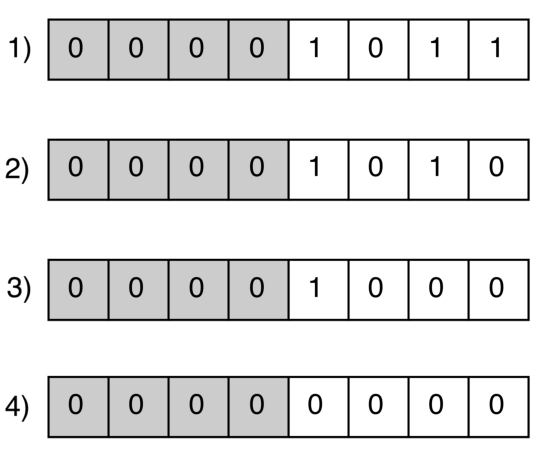
\includegraphics[width=\linewidth]{rxResponseMaskAnc.pdf}
      \end{center}
    \end{column}
    \begin{column}{0.7\textwidth}
      \begin{itemize}
      \item[1.] la maschera viene inizializzata all'arrivo del Poll in tutte le ancore mettendo a $0$ il bit corrispondente alla posizione dell'ancora master
      \item[2.] dopo che l'ancora $0$ ha risposto viene posto a $0$ il bit corrispondente alla posizione dell'ancora 
      \item[3.] dopo che l'ancora $1$ ha risposto viene posto a $0$ il bit corrispondente alla posizione dell'ancora 
      \item[4.] dopo che l'ancora $3$ ha risposto viene posto a $0$ il bit corrispondente alla posizione dell'ancora 
      \end{itemize}
    \end{column}
  \end{columns}
  \begin{exampleblock}{L'ancora i-esima decide di rispondere}
    quando è il primo bit (da destra) diverso da $0$ è il bit i-esimo.
  \end{exampleblock}
\end{frame}

\begin{frame}[fragile]{Header instance.h - Enum}
  Il seguente enum è stato modificato
  \begin{C}
    typedef enum instanceModes{LISTENER, TAG, TAG_WAIT, ANCHOR, ANCHOR_RNG, NUM_MODES} INST_MODE;
  \end{C}
  È stato aggiunto l'enumeratore \lstinline[language=C]!TAG_WAIT!. Esso corrisponde alla modalità in cui il tag
  attende il completamento della procedura di autoranging.
\end{frame}

\begin{frame}[shrink=10]{\lstinline!rxResponseMaskAnc! - Lato ancora \alert{non} master}
  L'invio delle risposte da parte delle ancore viene regolato dalla maschera \lstinline!rxResponseMaskAnc!.
  Viene mostrato un esempio in cui l'ancora $2$ si comporta da master.
  \begin{columns}
    \begin{column}{0.4\textwidth}
      \begin{center}
        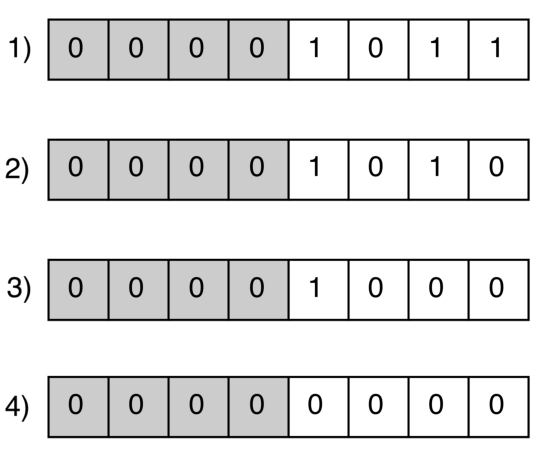
\includegraphics[width=\linewidth]{rxResponseMaskAnc.pdf}
      \end{center}
    \end{column}
    \begin{column}{0.7\textwidth}
      \begin{itemize}
      \item[1)] la maschera viene inizializzata all'arrivo del Poll in tutte le ancore mettendo a $0$ il bit corrispondente alla posizione dell'ancora master
      \item[2)] dopo che l'ancora $0$ ha risposto viene posto a $0$ il bit corrispondente alla posizione dell'ancora 
      \item[3)] dopo che l'ancora $1$ ha risposto viene posto a $0$ il bit corrispondente alla posizione dell'ancora 
      \item[4)] dopo che l'ancora $3$ ha risposto viene posto a $0$ il bit corrispondente alla posizione dell'ancora 
      \end{itemize}
    \end{column}
  \end{columns}
  \begin{exampleblock}{Regola generale}
    E' il turno dell'ancora i-esima di rispondere se il bit in posizione i-esima è il primo diverso da $0$ da destra 
  \end{exampleblock}
\end{frame}

\begin{frame}[shrink = 10]{File instance\_common.c}% - funzioni che gestiscono la maschera \lstinline!rxResponseMaskAnc!}
  \begin{block}{\lstinline!uint8 anch_has_responded()!}
    Restituisce \lstinline!True! se l'istanza ha già risposto altrimenti restituisce \lstinline!False!
  \end{block}
  \begin{block}{\lstinline!uint8 anch_tx_or_wait()!}
    Restituisce \lstinline!True! se l'istanza deve spedire la risposta al tag per poi aggiornare la maschera altrimenti restituisce \lstinline!False!\\
    \textcolor{dgreen}{Attenzione:} l'ancora i-esima deve rispondere se il bit in posizione i-esima della maschera \lstinline!rxResponseMaskAnc! è il primo bit diverso da $0$
    da destra
  \end{block}
  \begin{block}{\lstinline!void handle_rx_mask_on_timout()!}
    Funzione utilizzata per gestire un evento di TimeOut nella procedura di autoranging.\\
    Trova la posizione del primo bit uguale a $1$ nella maschera \lstinline!rxResponseMaskAnc!. La posizione di questo bit corrisponde all'indice dell'ancora che avrebbe
    dovuto inviare la risposta. Successivamente setta il bit a $0$ così da simulare l'avvenuta ricezione del messaggio.
  \end{block}
\end{frame}

\begin{frame}[fragile]{File instance\_common.c}
  \begin{block}{\lstinline!int eval_range(double* range, uint32 tof)!}
    Funzione utilizzata per convertire i tof in distanze espressi in \SI{}{\meter}. Restituisce $0$ se il risultato è negativo o maggiore di \SI{20}{\kilo\meter}, 
    $1$ altrimenti.
  \end{block}
  \begin{block}{\lstinline!void instanceclearcounts()!}
    Viene aggiunta l'inizializzazione di \lstinline!anchRngArray[i]! e \lstinline!tofAnc!
    dove $i$ varia da $0$ a \lstinline!MAX_ANCHOR_LIST_SIZE - 1!
    \begin{lstlisting}
      instance_data[0].anchRngArray[i] = INVALID_TOF;
      instance_data[0].tofAnc = INVALID_TOF;
    \end{lstlisting}
  \end{block}
\end{frame}

\begin{frame}[fragile]{File instance\_common.c}
  \begin{block}{\lstinline!void instanceclearcounts()!}
    Viene inizializzato il numero di volte che il Tag invia la sua posizione al Viewer.
    \begin{lstlisting}
      instance_data[0].tagPositionSentToViewer = 0;
    \end{lstlisting}
    \textcolor{dgreen}{Attenzione:} ogni \lstinline!SEND_ANCHOR_POSITION_EVERY_CYCLES! volte che il tag invia la sua posizione al Viewer tramite seriale viene inviata
    la posizione delle ancore
  \end{block}
  \begin{block}{\lstinline!void instance_set_anch_sleep_delay(int sleepdelay)!}
    Copia in \lstinline!anchSleepTime_ms! il periodo di trasmissione di ogni Poll da parte dell'ancora master
  \end{block}
\end{frame}

\begin{frame}{File instance\_common.c}
  \begin{block}{\lstinline!void enable_tag_polling(instance_data_t *inst)!}
    Inizializza il Tag per la normale procedura di ranging, le istruzioni contenute in questa funzione sono state
    prese dalla parte relativa al Tag del \lstinline!TA_INIT! originale
  \end{block}
\end{frame}

\begin{frame}[fragile]{File instance\_common.c}
  \begin{block}{\lstinline!void instance_backtoanchor(instance_data_t *inst)!}
    Funzione chiamata al termine della procedura di autoranging, oltre a resettare i Timeout
    \begin{lstlisting}
      dwt_setrxtimeout(0);
      dwt_setpreambledetecttimeout(0);
      dwt_setrxaftertxdelay(0);
    \end{lstlisting}
    si occupa di informare l'utente attraverso lo schermo LCD che la procedura di autoranging è terminata
    \begin{lstlisting}
      sprintf((char*)&buff[0], "A:%d AutoRng End", inst->instanceAddress16 & 0x3);
      writetoLCD(16, 1, buff);
    \end{lstlisting}
  \end{block}
\end{frame}

\begin{frame}[fragile]{File instance\_common.c}
  \begin{block}{\lstinline!void eval_means(instance_data_t *inst)!}
    Utilizzata per calcolare le medie dei range accumulati durante la fase di autoranging
    \begin{lstlisting}
      for(i = 0; i < MAX_ANCHOR_LIST_SIZE; i++)
      {
        if(i == (inst->instanceAddress16 & 0x3))
          continue;
        inst->anchRngArray[i] /= inst->anchRngArrayCounter[i];
      }
    \end{lstlisting}
    durante il calcolo della media \alert{non} viene considerato il range di un'ancora con se stessa
  \end{block}
\end{frame}

\begin{frame}[fragile,shrink=30]{File instance\_common.c}
  \begin{block}{\lstinline!void inst_processrxtimeout(instance_data_t *inst)!}
    Gestisce il comportamento dell'ancora master in caso di TimeOut.
    Qualora lo stato precedente fosse \lstinline!TA_TXPOLL_WAIT_SEND! prepara l'ancora all'invio di un nuovo Poll
    \begin{lstlisting}
      inst->instToSleep = TRUE;
      inst->testAppState = TA_TXE_WAIT;
      inst->nextState = TA_TXPOLL_WAIT_SEND;
    \end{lstlisting}
    Qualora lo stato precedente fosse \lstinline!TA_TXFINAL_WAIT_SEND! prepara l'ancora all'invio di un nuovo Poll    
    \begin{lstlisting}
      dwt_forcetrxoff();
      inst->instToSleep = TRUE;
      inst->testAppState = TA_TXE_WAIT;
      inst->nextState = TA_TXPOLL_WAIT_SEND;
    \end{lstlisting}
    Infine gestisce il comportamento dell'ancora \alert{non} master in caso di TimeOut riabilitando immediatamente la ricezione
    \begin{lstlisting}
      inst->testAppState = TA_RXE_WAIT;
      dwt_setrxtimeout(0);
    \end{lstlisting}
  \end{block}
\end{frame}

\begin{frame}[fragile, shirnk=30]{File instance\_common.c}
  \begin{block}{\lstinline!uint8 anc_rx_reenable()!}
    Funzione utilizzata per gestire il comportamento dell'ancora master ad ogni ricezione di un messaggio di risposta.\\
    La maschera \lstinline!mask!
    \begin{lstlisting}
    uint8 mask = (~(0x1 << instance_address)) & 0xF;
    \end{lstlisting}
    viene utilizzata per capire se tutte le ancore hanno risposto ed in quel caso l'istanza si prepara ad inviare il messaggio di Final.\\
    Nel caso in cui solo alcune risposte sono arrivate e \lstinline!instance_data[0].responseTO > 0! viene riconfigurato il TimeOut e riabilitata
    la ricezione 
    \begin{lstlisting}
    dwt_setrxtimeout(fwtoTime_sy * responseTO); 
    dwt_rxenable(DWT_START_RX_IMMEDIATE);
    \end{lstlisting}
  \end{block}
\end{frame}

\begin{frame}{File instance\_common.c}
  \begin{block}{\lstinline!uint8 anc_rx_reenable()!}
    Se, infine, secondo la maschera non tutti hanno risposto ma \lstinline!instance_data[0].responseTO <= 0! viene supposto che l'ultimo messaggio
    arrivato fosse corrotto e viene comunque inviato il Final così da permettere alle ancore che hanno risposto di calcolare il TOF
  \end{block}
  \begin{block}{\lstinline!uint8 anctxorrxreenable(uint16 sourceAddress)!}
    Eliminate le parti realtive alla procedura di autoranging già implementata nel firmware originario della DecaWave
  \end{block}
\end{frame}

\begin{frame}[fragile,shrink=30]{File instance\_common.c}
  \begin{block}{\lstinline!uint8 anc_tx_or_rxreenable_autoranging()!}
    Funzione utilizzata durante la procedura di autoranging dalle ancore non master.
    Qualora tutte le ancore avessero risposto (i.e. \lstinline!instance_data[0].rxResponseMaskAnc == 0!) l'istanza torna nuovamente in ricezione, disabilitando tutti i
    TimeOut, in attesa del messaggio di Final da parte dell'ancora master 
    \begin{lstlisting}
      dwt_setrxtimeout(0);
      dwt_setpreambledetecttimeout(0);
    \end{lstlisting}
    Se, invece è il suo turno di rispondere (i.e. \lstinline!anch_tx_or_wait() == True!) effettua un invio ritardato
    \begin{lstlisting}
      dwt_setdelayedtrxtime(instance_data[0].delayedReplyTime);
      dwt_starttx(DWT_START_TX_DELAYED | DWT_RESPONSE_EXPECTED);
    \end{lstlisting}
    Qualora non fosse ancora il momento di rispondere (i.e. \lstinline!anch_tx_or_wait() == False!) riabilita immediatamente la ricezione
    \begin{lstlisting}
      ancenablerx();
    \end{lstlisting}    
    \textcolor{dgreen}{Attenzione:} dopo aver chiamato \lstinline!anch_tx_or_wait()! la \lstinline!rxResponseMaskAnch! potrebbe essere cambiata ed essere diventata
    nulla, ossia tutti hanno risposto, in tal caso vengono disabilitati i timeout e l'istanza torna nuovamente in ricezione per attendere l'arrivo del messaggio di Final
  \end{block}
\end{frame}

\begin{frame}[fragile]{File instance\_common.c}
  \begin{block}{\lstinline!void handle_error_unknownframe(event_data_t dw_event)!}
    Nel caso in cui il tag sia in modalità \lstinline!TAG_WAIT! gestisce l'arrivo di un messaggio con modalità di indirizzamento
    errata oppure il fatto che \lstinline!rxd->event! sia diverso da \lstinline!DWT_SIG_RX_OKAY! e da \lstinline!DWT_SIG_RX_TIMEOUT!
    La chiamata a questa funzione comporta l'inserimento in coda di un evento di tipo \lstinline!TIMEOUT!)
    \begin{lstlisting}
      dwt_setrxtimeout(0);
      dwt_setpreambledetecttimeout(0);
      ...
      instance_putevent(dw_event, DWT_SIG_RX_TIMEOUT);
    \end{lstlisting}
  \end{block}
\end{frame}

\begin{frame}[fragile,shrink=20]{File instance\_common.c}
  \begin{block}{\lstinline!void ancprepareresponse(uint16 sourceAddress, uint8 srcAddr_index, uint8 fcode_index, uint8 *frame, uint32 uTimeStamp)!}
    E' stata rimossa la parte che gestiva la procedura di autoranging già implementata nel firmware della DecaWave. Vengono inoltre copiate nel messaggio
    di risposta che viene inviato al tag le medie dei range calcolate durante la procedura di autoranging
    \begin{lstlisting}
      for(i = anc_addr + 1, j = 0; i < MAX_ANCHOR_LIST_SIZE; i++, j++)
      {
        uint8 msg_index = AUTORANGING_RANGES + j * sizeof(double);
        memcpy(&(instance_data[0].msg_f.messageData[msg_index]), &instance_data[0].anchRngArray[i], sizeof(double));
      }
    \end{lstlisting}
    \begin{itemize}
    \item[-] l'ancora A$0$ invia i range $r_{0,1}$, $r_{0,2}$ e $r_{0,3}$
    \item[-] l'ancora A$1$ invia i range $r_{1,2}$ e $r_{1,3}$
    \item[-] l'ancora A$2$ invia il range $r_{2,3}$
    \end{itemize}
  \end{block}
\end{frame}

\begin{frame}{File instance\_common.c}
  \begin{block}{\lstinline!void anc_prepare_response_autoranging(uint8 srcAddr_index, uint8 fcode_index, uint8 *frame)!}
    Funzione utilizzata dalle ancore per prerare un messaggio di risposta durante la fase di autoranging.
  \end{block}
\end{frame}

\begin{frame}{File instance\_common.c}
  La funzione \lstinline!void instance_rxcallback(const dwt_callback_data_t *rxd)! ...
\end{frame}

\begin{frame}[fragile]{File instance\_common.c - funzione \lstinline!instance_rxcallback!}
  \begin{block}{fcode \lstinline!RTLS_DEMO_MSG_TAG_POLL!}
    Nel caso in cui un tag sia in modalità \lstinline!TAG_WAIT! inizia la normale procedura di ranging senza aspettare il timeout di $\SI{10}{\second}$
    \begin{lstlisting}
      enable_tag_polling(&instance_data[0]);
      instance_data[0].autoranging_timeout = FALSE;
    \end{lstlisting}
  \end{block}
\end{frame}

\begin{frame}[fragile, shrink=30]{File instance\_common.c - funzione \lstinline!instance_rxcallback!}
  \begin{block}{fcode \lstinline!RTLS_DEMO_MSG_ANCH_POLL!}
    Nel caso in cui un tag sia in modalità \lstinline!TAG_WAIT! sono settati a zero i timeout di ricezione
    \begin{lstlisting}
      dwt_setrxtimeout(0);
      dwt_setpreambledetecttimeout(0);
    \end{lstlisting}
    Nel caso in cui il messaggio sia ricevuto da un'ancora in modalità \lstinline!ANCHOR_RNG! viene settata la maschera
    \lstinline!rxResponseMaskAnc!
    \begin{lstlisting}
      instance_data[0].rxResponseMaskAnc = (~(0x1 << master_anchor)) & 0xF;    
    \end{lstlisting}
    viene preparata la risposta con l'ultimo TOF calcolato
    \begin{lstlisting}
      anc_prepare_response_autoranging(srcAddr_index, fcode_index, &dw_event.msgu.frame[0]);
    \end{lstlisting}
    configurato il timeout 
    \begin{lstlisting}
      dwt_setrxtimeout((uint16)instance_data[0].fwtoTimeAnc_sy);
    \end{lstlisting}
    e gestito l'invio del messaggio
    \begin{lstlisting}
      anc_tx_or_rxreenable_autoranging(instance_data[0].instanceAddress16);
    \end{lstlisting}
  \end{block}
\end{frame}

\begin{frame}[fragile, shrink=50]{File instance\_common.c - funzione \lstinline!instance_rxcallback!}
  \begin{block}{fcode \lstinline!RTLS_DEMO_MSG_ANCH_RESP2!}
    Nel caso in cui un tag sia in modalità \lstinline!TAG_WAIT! sono settati a zero i timeout di ricezione
    \begin{lstlisting}
      dwt_setrxtimeout(0);
      dwt_setpreambledetecttimeout(0);
    \end{lstlisting}
    Nel caso in cui il messaggio sia ricevuto da un'ancora \alert{master} in modalità \lstinline!ANCHOR_RNG! e viene aggiornata la maschera
    e decrementato il contatore
    \begin{lstlisting}
      instance_data[0].responseTO--;
      instance_data[0].rxResponseMaskAnc |= (0x1 << (sourceAddress & 0x3));
    \end{lstlisting}
    Viene inoltre gestito il comportamento dell'ancora \alert{master} (i.e. continua ad aspettare ed invia il messaggio di Final)
    \begin{lstlisting}
      anc_rx_reenable();
    \end{lstlisting}
    Nel caso in cui il messaggio sia ricevuto da un'ancora \alert{non} master in modalità \lstinline!ANCHOR_RNG! la cui maschera sia
    diversa da $0$ (i.e. non sono state ricevute tutte le risposte dalle altre ancore) \lstinline!ANCHOR_RNG! viene aggiornata e l'invio del
    messaggio viene gestito
    \begin{lstlisting}
      instance_data[0].rxResponseMaskAnc &= ~(0x1 << (sourceAddress & 0x3));
      anc_tx_or_rxreenable_autoranging();
    \end{lstlisting}
    Il caso in cui la maschera fosse completamente nulla l'istanza potrebbe non aver ricevuto un messaggio di Poll oppure tutte le risposte sono state già
    ricevute, in questo caso viene resettato il TimeOut e riabilitata immediatamente la ricezione
    \begin{lstlisting}
      dwt_setrxtimeout(0);
      dwt_rxenable(DWT_START_RX_IMMEDIATE);
    \end{lstlisting}
  \end{block}
\end{frame}

\begin{frame}[fragile]{File instance\_common.c - funzione \lstinline!instance_rxcallback!}
  \begin{block}{condizione \lstinline!rxd->event == DWT_SIG_RX_TIMEOUT!}
    Nel caso in cui un'ancora \alert{non} master in modalità \lstinline!ANCHOR_RNG! non abbia ricevuto la risposta attesa e il TimeOut sia scattato viene
    aggiornata la \lstinline!rxResponseMaskAnc! e, nel caso sia arrivato il turno per l'istanza di inviare la risposta, risponde all'ancora master. Così
    da preservare l'interazione tra l'istanza e l'ancora master e calcolare comunque il nuovo TOF
    \begin{lstlisting}
      handle_rx_mask_on_timout();
      anc_tx_or_rxreenable_autoranging();
    \end{lstlisting}
    Viene inoltre generato un evento di tipo \lstinline!DWT_SIG_RX_TIMEOUT!
    \begin{lstlisting}
      instance_putevent(dw_event, DWT_SIG_RX_TIMEOUT);
    \end{lstlisting}
  \end{block}
\end{frame}

\begin{frame}[fragile]{File instance\_common.c}
  \begin{block}{\lstinline!int instance_run()!}
    Nel caso in cui l'uscita della macchina a stati sia \lstinline!INST_DONE_WAIT_FOR_NEXT_EVENT_TO! viene reimpostato il TimeOut per l'invio di un nuovo Poll
    da parte dell'ancora \alert{master}
    \begin{lstlisting}
      nextPeriod = instance_data[0].anchSleepTime_ms;
      instance_data[0].nextSleepPeriod = (uint32) nextPeriod;
    \end{lstlisting}
    Nel caso \lstinline!TAG_WAIT! viene gestito il TimeOut che consente di iniziare la normale procedura di ranging quando
    non viene più rilevata attività di autoranging
    \begin{lstlisting}
      enable_tag_polling(&instance_data[0]);
      instance_data[instance].autoranging_timeout = FALSE;
    \end{lstlisting}
  \end{block}
\end{frame}


    

\section{instance.c}
\begin{frame}[fragile]{File instance.c - \lstinline[language=C]!testapprun!}
  La funzione
  \begin{C}
    int testapprun(instance_data_t *inst, int message)
  \end{C}
  contiene una macchina a stati che implementa la logica di funzionamento delle ancore e dei tag.
  Essa è stata modificata al fine di rimuovere la vecchia modalità di autoranging ed inserire la nuova.\\
  Nel seguito sono descritti i principali \alert{cambiamenti} apportati.
\end{frame}

\begin{frame}[fragile]{File instance.c - \lstinline[language=C]!testapprun!}
  \begin{block}{Stato \lstinline[language=C]!TA_INIT!}
    Un tag in modalità \lstinline[language=C]!TAG_WAIT! abilita la ricezione di eventuali messaggi
    provenienti dalle ancore che eseguono l'autoranging.\\
    Il codice
    \begin{C}
      inst->autoranging_timeout = TRUE;
      inst->autoranging_poll_time = portGetTickCount();
    \end{C}
    abilita il timeout software utilizzato per attendere la fine della procedura di autoranging e
    memorizza l'istante di tempo corrente nel caso in cui la procedura di autoranging fosse terminata
    prima dell'accensione del tag.
  \end{block}
\end{frame}

\begin{frame}[fragile]{File instance.c - \lstinline[language=C]!testapprun!}
  \begin{block}{Stato \lstinline[language=C]!TA_INIT! - continuazione}
    Di solito, infatti, \lstinline[language=C]!autoranging_poll_time! viene assegnato
    alla ricezione da parte del tag di un Poll inviato da un'ancora master.\\
    Il codice
    \begin{C}
      inst->autoRngRangesRxMask = 0;
    \end{C}
    inizializza la maschera che indica da quali ancore il tag ha ricevuto i range medi.\\
    \alert{Lo stato successivo} è \lstinline[language=C]!TA_RXE_WAIT!.
  \end{block}
\end{frame}

\begin{frame}[fragile]{File instance.c - \lstinline[language=C]!testapprun!}
  \begin{block}{Stato \lstinline[language=C]!TA_INIT! - continuazione}
    Un'ancora in modalità \lstinline[language=C]!ANCHOR_RNG! si comporta diversamente a seconda che sia l'ancora master o meno.\\
    L'ancora A0 viene configurata come ancora master e preparata per eseguire il primo sleep prima dell'invio del primo Poll.
    Il codice
    \begin{C}
      for(i=0; i<MAX_ANCHOR_LIST_SIZE; i++)
          inst->anchRngArrayCounter[i] = 0;
      
      uint16 instance_address = inst->instanceAddress16 & 0x3;
      inst->anchRngArrayCounter[instance_address] = 0xFFFF - 0x1;
    \end{C}
    si occupa di inizializzare il contatore delle misure raccolte per ogni range di interesse.
  \end{block}
\end{frame}


\begin{frame}[fragile]{File instance.c - \lstinline[language=C]!testapprun!}
  \begin{block}{Stato \lstinline[language=C]!TA_INIT! - continuazione}
    Per ogni ancora master, sia l'$i$-esima, $i \ge 0$, il ruolo di ancora master si considera terminato
    quando l'elemento più piccolo dell'array \lstinline[language=C]!anchRngArrayCounter! è maggiore o uguale a
    \lstinline[language=C]!NUM_AUTORNG_RGN!. Dal momento che l'elemento $i$-esimo dell'array, che si riferisce al range
    $r_{ii}$, non viene mai aggiornato esso viene posto al massimo numero rappresentabile su $16$ bit.\\
    \alert{Lo stato successivo} è \lstinline[language=C]!TA_TXE_WAIT!.
  \end{block}
\end{frame}

\begin{frame}[fragile]{File instance.c - \lstinline[language=C]!testapprun!}
  \begin{block}{Stato \lstinline[language=C]!TA_INIT! - continuazione}
    Le altre ancore, con indirizzo diverso da A0, abilitano la ricezione
    e rimangono in attesa di messaggi di Poll inviati dall'ancora master.\\
    \alert{Lo stato successivo} è \lstinline[language=C]!TA_RXE_WAIT!.
  \end{block}
\end{frame}

\begin{frame}[fragile, shrink=10]{File instance.c - \lstinline[language=C]!testapprun!}
  \begin{block}{Stato \lstinline[language=C]!TA_SLEEP_DONE!}
    In questo stato i tag, nel loro funzionamento normale, e le ancore master, in modalità
    \lstinline[language=C]!ANCHOR_RNG!, attendono che sia il momento di inviare un nuovo Poll.\\
    Per le ancore è stato deciso di non utilizzare la modalità \lstinline[language=C]!DEEP_SLEEP!
    per cui, pur entrando nel ramo \lstinline[language=C]!DEEP_SLEEP == 1!, viene replicata l'istruzione
    \lstinline[language=C]!Sleep(3)! prevista nel ramo \lstinline[language=C]!#else!.
    \begin{C}
      #if (DEEP_SLEEP == 1)
          if (inst->mode == TAG)
          {
            ...
          }  
          else if (inst->mode == ANCHOR_RNG)
              Sleep(3);
      #else
          Sleep(3);
      #endif
    \end{C}
  \end{block}
\end{frame}

\begin{frame}[fragile, shrink=10]{File instance.c - \lstinline[language=C]!testapprun!}
  \begin{block}{Stato \lstinline[language=C]!TA_TXE_WAIT!}
    In questo stato i tag, nel loro funzionamento normale, e le ancore master, in modalità
    \lstinline[language=C]!ANCHOR_RNG!, eseguono alcune operazioni in preparazione alla spedizione
    del successivo Poll.\\
    In particolare con le istruzioni
    \begin{C}
      if (inst->mode == ANCHOR_RNG)
          inst->rangeNumAnc++;
      ...
      else if (inst->mode == ANCHOR_RNG)
          inst->rxResponseMaskAnc = 0;
    \end{C}
    l'ancora master, replicando il comportamento di un tag, incrementa il rangeNumber,
    utilizzato nel protocollo di trasmissione per eseguire un integrity check, e riporta
    a zero la maschera che indica quali ancore hanno risposto al Poll inviato.
  \end{block}
\end{frame}

\begin{frame}[fragile, shrink=10]{File instance.c - \lstinline[language=C]!testapprun!}
  \begin{block}{Stato \lstinline[language=C]!TA_TX_POLL_WAIT_SEND!}
    In questo stato i tag, nel loro funzionamento normale, e le ancore master, in modalità
    \lstinline[language=C]!ANCHOR_RNG!, spediscono effettivamente il Poll.\\
    In particolare con le istruzioni
    \begin{C}
      inst->responseTO = MAX_ANCHOR_LIST_SIZE - 1;
      dwt_setrxtimeout((uint16)inst->fwtoTime_sy * (MAX_ANCHOR_LIST_SIZE - 1));
    \end{C}
    l'ancora master, replicando il comportamento di un tag, configura un timeout di ricezione
    di durata proporzionale al numero di risposte attese \lstinline[language=C]!MAX_ANCHOR_LIST_SIZE - 1!.
    Tale numero è inferiore di uno rispetto al numero di risposte attese normalmente da un tag
    dato che una delle ancore si comporta come master.
  \end{block}
\end{frame}

\begin{frame}[fragile]{File instance.c - \lstinline[language=C]!testapprun!}
  \begin{block}{Stato \lstinline[language=C]!TA_TX_FINAL_WAIT_SEND!}
    In questo stato i tag, nel loro funzionamento normale, e le ancore master, in modalità
    \lstinline[language=C]!ANCHOR_RNG!, spediscono effettivamente il Final.\\
    Dato che l'ancora master invia un byte in più per specificare se il \alert{proprio} ruolo di ancora master
    è terminato è necessario modificare la lunghezza del messaggio con l'istruzione
    \begin{C}
      inst->psduLength = (ANCH_FINAL_MSG_LEN + FRAME_CRTL_AND_ADDRESS_S + FRAME_CRC);
    \end{C}
    dove \lstinline[language=C]!ANCH_FINAL_MSG_LEN! vale $34$ invece che $33$ come nel caso del tag.
  \end{block}
\end{frame}

\begin{frame}[fragile]{File instance.c - \lstinline[language=C]!testapprun!}
  \begin{block}{Stato \lstinline[language=C]!TA_TX_FINAL_WAIT_SEND! - continuazione}
    Con le istruzioni
    \begin{C}
      inst->msg_f.messageData[END_AUTORANGING] = FALSE;
      ...
      if(inst->mode == ANCHOR_RNG && 
      array_min(inst->anchRngArrayCounter, MAX_ANCHOR_LIST_SIZE) >= NUM_AUTORNG_RNG)
      {
        inst->anchorRngMaster++;
        inst->msg_f.messageData[END_AUTORANGING] = TRUE;
      }
    \end{C}
    viene modificato il flag che indica se il ruolo di ancora master è terminato e viene
    incrementata la variabile contenente l'ID dell'ancora master corrente.
  \end{block}
\end{frame}

\begin{frame}[fragile, shrink=30]{File instance.c - \lstinline[language=C]!testapprun!}
  \begin{block}{Stato \lstinline[language=C]!TA_TX_FINAL_WAIT_CONF!}
    In questo stato i tag, nel loro funzionamento normale, e le ancore master, in modalità
    \lstinline[language=C]!ANCHOR_RNG!, verificano l'avvenuta spedizione del Poll e del Final.\\
    Per quanto riguarda l'ancora master, nel caso in cui stia verificando l'avvenuta spedizione
    di un Poll, si comporta come un tag.\\
    Se invece l'ancora master sta verificando la spedizione di un Final e viene soddisfatto il criterio
    di termine del proprio ruolo di ancora master allora si porta nello stato di ricezione
    \lstinline[language=C]!TA_RXE_WAIT! in cui attenderà la ricezione di nuovi Poll provenienti dalla nuova ancora master.
    \begin{C}
      if(inst->previousState == TA_TXFINAL_WAIT_SEND)
      {
        if(inst->mode == ANCHOR_RNG && 
        array_min(inst->anchRngArrayCounter, MAX_ANCHOR_LIST_SIZE) >= NUM_AUTORNG_RNG)
        {
          ...
          inst->testAppState = TA_RXE_WAIT;
          ...
    \end{C}
  \end{block}
\end{frame}

\begin{frame}[fragile, shrink=30]{File instance.c - \lstinline[language=C]!testapprun!}
  \begin{block}{Stato \lstinline[language=C]!TA_TX_FINAL_WAIT_CONF! - continuazione}
    Inoltre se, dopo aver incrementato il contatore \lstinline[language=C]!anchorRngMaster!,
    l'indirizzo della nuova ancora master è pari
    al numero totale di ancore allora la procedura \alert{complessiva} di autoranging
    è terminata ed è possibile ripristinare la modalità normale di funzionamento \lstinline[language=C]!ANCHOR!
    attraverso la chiamata alla funzione \lstinline[language=C]!instance_backtoanchor()!.
    \begin{C}
          if((inst->anchorRngMaster & 0x7) == MAX_ANCHOR_LIST_SIZE))
            instance_backtoanchor(inst);
          ...
          }
    \end{C}
    \alert{Solo l'ultima ancora} chiama la funzione \lstinline[language=C]!instance_backtoanchor()!
    in questa parte della macchina a stati. Le altre ancore rilevano il termine della procedura
    di autoranging quando ricevono l'ultimo final inviato dall'ultima
    ancora nello stato \lstinline[language=C]!TA_RX_WAIT_DATA!.
  \end{block}
\end{frame}

\begin{frame}{File instance.c - \lstinline[language=C]!testapprun! - \lstinline[language=C]!TA_RX_WAIT_DATA!}
  Lo stato \lstinline[language=C]!TA_RX_WAIT_DATA!, assieme alla callback di ricezione \lstinline[language=C]!instance_rxcallback()!
  contenuta nel file \lstinline[language=C]!instance_common.c!, si occupa di processare i messaggi ricevuti dal dispositivo,
  ancora o tag, e ne modifica il comportamento di consenguenza.\\
  Nel caso in cui il dispositivo abbia ricevuto un messaggio valido, lo stato \lstinline[language=C]!TA_RX_WAIT_DATA!
  prevede comportamenti diversi in base all'\lstinline[language=C]!FCODE! contenuto nel messaggio.\\
  Di seguito sono descritti i principali \alert{cambiamenti} apportati a questo stato suddivisi
  per \lstinline[language=C]!FCODE!.
\end{frame}

\begin{frame}[fragile, shrink=30]{File instance.c - \lstinline[language=C]!testapprun! - \lstinline[language=C]!TA_RX_WAIT_DATA!}
  Il firmware originale gestiva gli fcode \lstinline[language=C]!RTLS_DEMO_MSG_TAG_POLL! e
  \lstinline[language=C]!RTLS_DEMO_MSG_ANCH_POLL! assieme. Nella nuova release sono gestiti separatamente.
  \begin{block}{fcode \lstinline[language=C]!RTLS_DEMO_MSG_ANCH_POLL!}
    Le ancore che ricevono un Poll da parte di un'ancora master si comportano come le ancore
    che ricevono un Poll da parte di un tag nella normale procedura di ranging.\\
    Un tag nella modalità \lstinline[language=C]!TAG_WAIT! reimposta il tempo di ricezione del Poll in modo
    da garantire il funzionamento del sistema di timeout con cui il tag si rende conto del termine
    della procedura di autoranging. In questa situazione il tag torna ad ascoltare nello stato
    \lstinline[language=C]!TA_RXE_WAIT!.
    \begin{C}
      ...
      if (inst->mode == TAG_WAIT)
      {
        inst->autoranging_poll_time = portGetTickCount();
        inst->testAppState = TA_RXE_WAIT;

        break;
      }
      ...
    \end{C}
  \end{block}
\end{frame}

\begin{frame}[fragile]{File instance.c - \lstinline[language=C]!testapprun! - \lstinline[language=C]!TA_RX_WAIT_DATA!}
  Il firmware originale gestiva gli fcode \lstinline[language=C]!RTLS_DEMO_MSG_ANCH_RESP! e \lstinline[language=C]!_RESP2!
  assieme. Nella nuova release sono gestiti separatamente.
  \begin{block}{fcode \lstinline[language=C]!RTLS_DEMO_MSG_ANCH_RESP!}
    Il tag che riceve una risposta da parte di un'ancora si occupa anche di gestire i range medi
    elaborati durante la fase di autoranging e che ogni ancora si occupa di inviare al tag in risposta
    ad un Poll (oltre al Tof come previsto nel funzionamento normale della procedura di ranging).\\
    In particolare se il tag non ha aveva ancora ricevuto i range medi dall'ancora avente indirizzo
    \lstinline[language=C]!srcAddr[0]! quando ciò accade
    \begin{C}
      if ((inst->mode == TAG) && (inst->autoRngRangesRxMask & (0x1 << (srcAddr[0]&0x3))) == 0)
      {
    \end{C}
  \end{block}
\end{frame}

\begin{frame}[fragile]{File instance.c - \lstinline[language=C]!testapprun! - \lstinline[language=C]!TA_RX_WAIT_DATA!}
  \begin{block}{fcode \lstinline[language=C]!RTLS_DEMO_MSG_ANCH_RESP! - continuazione}
    valuta il numero di range che si aspetta di ricevere da tale ancora
    \begin{C}
        uint8 number_of_ranges = MAX_ANCHOR_LIST_SIZE - 1 - (srcAddr[0]&0x3);
    \end{C}
    e copia i dati dal messaggio appena ricevuto nella struttura dati \lstinline[language=C]!autoRngRangesArray!
    a partire dal byte \lstinline[language=C]!offset!-esimo.
    \begin{C}
        uint8 offset = 0;
        for(i = 0; i < (srcAddr[0]&0x3); i++)
          offset += (MAX_ANCHOR_LIST_SIZE - 1 - i);

        memcpy(&(inst->autoRngRangesArray[offset]), &(messageData[AUTORANGING_RANGES]),
        sizeof(double) * number_of_ranges);
    \end{C}
  \end{block}
\end{frame}

\begin{frame}[fragile, shrink=15]{File instance.c - \lstinline[language=C]!testapprun! - \lstinline[language=C]!TA_RX_WAIT_DATA!}
  \begin{block}{fcode \lstinline[language=C]!RTLS_DEMO_MSG_ANCH_RESP! - continuazione}
    Inoltre aggiorna la maschera \lstinline[language=C]!autoRngRangesRxMask! in modo da non ripetere
    la procedura di salvataggio dei range medi alla ricezione di altre risposte dalla medesima ancora.
    \begin{C}
        inst->autoRngRangesRxMask |= (0x1 << (srcAddr[0]&0x3));
    \end{C}
    Se il tag ha ricevuto tutti i range medi da tutte le ancora valuta le posizioni cartesiane
    delle ancore attraverso la chiamata alla funzione \lstinline[language=C]!rangeToPos! che salva il risultato
    nella matrice \lstinline[language=C]!anchorPositionMatrix!.
    \begin{C}
        if (inst->autoRngRangesRxMask  == (0x1 << MAX_ANCHOR_LIST_SIZE) - 1)
        {
          rangesToPos(inst->autoRngRangesArray,\
          inst->anchorPositionMatrix);
        }
      }
      ...
    \end{C}
  \end{block}
\end{frame}

\begin{frame}[fragile, shrink=15]{File instance.c - \lstinline[language=C]!testapprun! - \lstinline[language=C]!TA_RX_WAIT_DATA!}
  \begin{block}{fcode \lstinline[language=C]!RTLS_DEMO_MSG_ANCH_RESP2!}
    Un tag in \lstinline[language=C]!TAG_WAIT! ignora il messaggio riabilita la ricezione.\\
    Le ancore, master o meno, si comportano come in una normale procedura di ranging
    eccetto per il fatto che l'ancora master salva il tof ricevuto in un accumulatore
    \lstinline[language=C]!anchRngArray! e incrementa il contatore \lstinline[language=C]!anchRngArrayCounter!.
    \begin{C}
      ...
      if (inst->anchRngArrayCounter[src_addr] == 0)
        inst->anchRngArray[src_addr] = range;
      else 
        inst->anchRngArray[src_addr] += range;
      inst->anchRngArrayCounter[src_addr]++;
      ...
    \end{C}
  \end{block}
\end{frame}

\begin{frame}[fragile]{File instance.c - \lstinline[language=C]!testapprun! - \lstinline[language=C]!TA_RX_WAIT_DATA!}
  \begin{block}{fcode \lstinline[language=C]!RTLS_DEMO_MSG_TAG_FINAL! e \lstinline[language=C]!RTLS_DEMO_MSG_ANCH_FINAL!}
    Un tag in \lstinline[language=C]!TAG_WAIT! riabilita la ricezione.\\
    Un'ancora non master che riceve un \lstinline[language=C]!ANCH_FINAL! calcola il tof, come
    farebbe nel caso in cui ha ricevuto un \lstinline[language=C]!TAG_FINAL!, lo salva in un accumulatore
    \lstinline[language=C]!anchRngArray! ed incrementa il contatore \lstinline[language=C]!anchRngArrayCounter!
    \begin{C}
      if (inst->anchRngArrayCounter[src_addr] == 0)
        inst->anchRngArray[src_addr] = range;
      else 
        inst->anchRngArray[src_addr] += range;
      inst->anchRngArrayCounter[src_addr]++;
    \end{C}
  \end{block}
\end{frame}

\begin{frame}[fragile]{File instance.c - \lstinline[language=C]!testapprun! - \lstinline[language=C]!TA_RX_WAIT_DATA!}
  \begin{block}{fcode \lstinline[language=C]!RTLS_DEMO_MSG_ANCH_FINAL! - continuazione}
    Inoltre l'ancora verifica se il messaggio di Final ricevuto contiene
    il byte che indica la fine del ruolo di ancora master per l'ancora
    master corrente. Nel caso in cui la procedura sia terminata viene incrementato
    l'indirizzo dell'ancora master corrente. Inoltre \alert{viene invalidato} il tof
    dal momento che non potrebbe essere utilizzato nella risposta ad un Poll proveniente
    dalla successiva ancora master dato che è riferito all'ancora master precedente.
    \begin{C}
      if(messageData[END_AUTORANGING] == TRUE)
      {
        inst->anchorRngMaster++;
        inst->autoranging_timeout = FALSE;
        inst->tofAnc = INVALID_TOF;
      }
    \end{C}
  \end{block}
\end{frame}

\begin{frame}[fragile, shrink=30]{File instance.c - \lstinline[language=C]!testapprun! - \lstinline[language=C]!TA_RX_WAIT_DATA!}
  \begin{block}{fcode \lstinline[language=C]!RTLS_DEMO_MSG_ANCH_FINAL! - continuazione}
    Qualora l'ancora che ha ricevuto il final fosse la nuova ancora master
    si prepara per spedire il suo primo Poll (le inizializzazioni sono le medesime
    eseguite dall'ancora 0 nello stato \lstinline[language=C]!TA_INIT!).
    \begin{C}
      if(inst->mode == ANCHOR_RNG && inst->instanceAddress16 == inst->anchorRngMaster)
      {
        ...
        inst->autoranging_timeout = FALSE;
        inst->nextState = TA_TXPOLL_WAIT_SEND;
        inst->testAppState = TA_TXE_WAIT;
        
        inst->rangeNumAnc = 0;

        for(i=0; i<MAX_ANCHOR_LIST_SIZE; i++)
            inst->anchRngArrayCounter[i] = 0;

        uint16 instance_address = inst->instanceAddress16 & 0x3;
        inst->anchRngArrayCounter[instance_address] = 0xFFFF - 0x1;
        ...
      }
    \end{C}
  \end{block}
\end{frame}

\begin{frame}[fragile]{File instance.c - \lstinline[language=C]!testapprun! - \lstinline[language=C]!TA_RX_WAIT_DATA!}
  \begin{block}{fcode \lstinline[language=C]!RTLS_DEMO_MSG_ANCH_FINAL! - continuazione}
    Se al contrario l'ancora rileva che l'intera procedura di autoranging è completata,
    poichè l'indirizzo della nuova ancora master è pari al numero totale di ancore, calcola le medie
    dei range attraverso la funzione \lstinline[language=C]!eval_means()! e ripristina la modalità normale di funzionamento
    \lstinline[language=C]!ANCHOR! attraverso la funzione \lstinline[language=C]!instance_backtoanchor()!.
    \begin{C}
      ...
      else if((inst->mode == ANCHOR_RNG) && (inst->anchorRngMaster & 0x7) == MAX_ANCHOR_LIST_SIZE)
      {
        eval_means(inst);
        instance_backtoanchor(inst);
      }
      ...
    \end{C}
  \end{block}
\end{frame}

\begin{frame}[fragile]{File instance.c - \lstinline[language=C]!array_min!}
  La seguente funzione è stata aggiunta
  \begin{block}{\lstinline[language=C]!uint16 array_min (uint16* array, int len)!}
    Calcola il minimo di un array.
  \end{block}
\end{frame}

\begin{frame}[fragile, shrink=15]{File main.c}
  Nel seguito sono riportate alcune note riguardanti il file \lstinline!main.c!
  \begin{block}{Configurazione Slot and Superframe}
    In generale è stato aggiunto il campo relativo al periodo di trasmissione dei Poll
    da parte di un'ancora master. È stato verificato sperimentalmente che un periodo di \SI{10}{\milli\second} è
    sufficiente a gestire 4 ancore di cui una master.\\
    \begin{lstlisting}
      sfConfig_t sfConfig[4] =
      {
      ...
      //mode 2 - S1: 2 on, 3 off
      {
        (10),   // slot period (ms)
        (1),    // number of slots
        (10*1), // superframe period (ms)
        (10*1), // poll sleep delay (ms)
        (10),   // anch sleep delay in autoranging (ms)
        (2500)  // final transmission delay
      },
      ...
    };
  \end{lstlisting}
  \end{block}
\end{frame}

\begin{frame}[fragile, shrink=15]{File main.c}
  \begin{block}{\lstinline!uint32 inittestapplication(uint8 s1switch)!}
    La modalità di funzionamento di un dispositivo DecaWaveEVB1000 dipende
    dallo switch $n.4$ presente sul PCB.\\
    Un dispositivo di tipo tag, nella nuova release, non viene più inizializzato in modalità
    \lstinline!TAG! ma \lstinline!TAG_WAIT!. In tale modalità attende il termine della procedura
    di autoranging.\\
    Un dispositivo di tipo ancora, nella nuova release, non viene più inizializzato in modalità
    \lstinline!ANCHOR! ma \lstinline!ANCHOR_RNG!. In tale modalità le ancore eseguono la procedura
    di autoranging.
    \begin{lstlisting}
    if((s1switch & SWS1_ANC_MODE) == 0)
    {
      instance_mode = TAG_WAIT;
    }
    else
    {
      instance_mode = ANCHOR_RNG;
    }
    \end{lstlisting}
  \end{block}
\end{frame}

\begin{frame}[fragile, shrink=15]{File main.c}
  \begin{block}{\lstinline!void setLCDline1(uint8 s1switch)!}
    Questa funzione gestisce il testo riportato sul display LCD a seconda
    della modalità del dispositivo DecaWaveEVB1000.\\
    Nella nuova release del firmware i tag all'accensione riportano la scritta
    ``Waiting...'' ad indicare che attende il termine della procedura di autoranging.
    Le ancore invece riportano la scritta ``Autoranging''.
    \begin{lstlisting}
      ...
      else if(role == TAG_WAIT)
      {
        sprintf((char*)&dataseq1[0], "Tag:%d Waiting...", tagaddr);
        writetoLCD( 16, 1, dataseq1);
      }
      ...
      else if(role == ANCHOR_RNG)
      {
        sprintf((char*)&dataseq1[0], "A:%d Autoranging", ancaddr);
        writetoLCD( 16, 1, dataseq1);
      }
      ...
    \end{lstlisting}
  \end{block}
\end{frame}

\begin{frame}[fragile, shrink=30]{File main.c}
  \begin{block}{\lstinline!int main(void)!}
    Rispetto alla release precedente, il tag, dopo aver ricevuto i tof da tutte le ancore,
    invia il risulutato della trilaterazione attraverso la porta seriale (USB OTG VCP)
    \begin{lstlisting}
    ...  
    if(rx == TOF_REPORT_T2A)
    {
      if (instance_data[0].mode == TAG)
      {
        ...
        instance_data[0].tagPositionSentToViewer++;

  	 float pos_x = (float) best_solution.x;
	 float pos_y = (float) best_solution.y;
	 float pos_z = (float) best_solution.z;
	 print_over_otg_usb("tpr %d %08x %08x %08x",
                            (instance_data[0].instanceAddress16 & 0x7),
	                    *(uint32_t*)&pos_x,
                            *(uint32_t*)&pos_y,
                            *(uint32_t*)&pos_z);
    \end{lstlisting}
  \end{block}
\end{frame}

\begin{frame}[fragile, shrink=30]{File main.c}
  \begin{block}{\lstinline!int main(void)! - continuazione}
    Inoltre ogni \lstinline!SEND_ANCHOR_POSITION_EVERY_CYCLES! cicli invia sulla medesima
    porta la posizione cartesiana delle ancore.
    \begin{lstlisting}
	  if(instance_data[0].tagPositionSentToViewer == SEND_ANCHOR_POSITION_EVERY_CYCLES)
	  {
	    instance_data[0].tagPositionSentToViewer = 0;
	    print_over_otg_usb("apr %d %08x %08x %08x %08x %08x %08x %08x %08x %08x %08x %08x %08x",
			       (instance_data[0].instanceAddress16 & 0x7),
	                        *(uint32_t*)&(instance_data[0].
                                anchorPositionMatrix[0][0]),
			        ...
			        *(uint32_t*)&(instance_data[0].
                                anchorPositionMatrix[2][3]));
	  }
          ...
        }
        \end{lstlisting}
  \end{block}
\end{frame}

\begin{frame}[fragile]{Files autoranging.c e autoranging.h}
  La funzione
  \begin{C}
    int rangesToPos(double* ranges, float anch_position[][4])
  \end{C}
  è stata implementata sfruttando l'algoritmo algebrico di calibrazione sviluppato da Federica Fioretti.
\end{frame}

\begin{frame}[fragile]{File trilat.c}
  La funzione
  \begin{C}
    int computePosition_mm(float d1,float d2,float d3,float d4, vec3d *best_solution2, float anch_position[][4])
  \end{C}
  utilizza la posizione delle ancore in $\SI{}{\meter}$ calcolate mediante la funzione \lstinline[languace=C]!rangesToPos!
  \begin{C}
    // Anchor i
    pi.x = anch_position[0][i];
    pi.y = anch_position[1][i];
    pi.z = anch_position[2][i];
  \end{C}
\end{frame}
  


\section{algebric\_trilat.c}
\begin{frame}[fragile]{File algebric\_trilat.c}
  La funzione
  \begin{C}
    int computePosition_mm(float d1,float d2,float d3,float d4, vec3d *best_solution2, float anch_position[][4])
  \end{C}
  utilizza, rispetto al passato, la posizione delle ancore in $\SI{}{\milli\meter}$ calcolate mediante la funzione \lstinline[language=C]!rangesToPos!
  \begin{C}
    for(index = 0; index<3; index++)
    {
      A_mm[index] = anch_position[index][0] * 1000;
      B_mm[index] = anch_position[index][1] * 1000;
      C_mm[index] = anch_position[index][2] * 1000;
      D_mm[index] = anch_position[index][3] * 1000;
    }
  \end{C}
\end{frame}

\begin{frame}[fragile]{File print\_over\_otg\_usb.c}
  La funzione
  \begin{C}
    void print_over_otg_usb(const char * format, ...)
  \end{C}
  permette di inviare una stringa, utilizzando il formato della funzione \lstinline[language=C]!printf()!, tramite la porta USB OTG.
\end{frame}



\end{document}
